%-----------------------------------------------------------------------------
\documentclass[12pt,a4paper]{report}
%-----------------------------------------------------------------------------
\usepackage{amsmath}
\usepackage{amssymb}
\usepackage{amsthm}
% enumitem is loaded for the web build: without it tex4ht discards the
% optional label on \item[(i)] and numbers the list itself, so remarks
% labelled (i), (ii), (iii) come out as 1, 2, 3 and cross-references break.
\usepackage{enumitem}
\usepackage{array}
\usepackage{longtable}
\usepackage{appendix}
\usepackage{blkarray}
\usepackage{bibentry}
\usepackage[noadjust]{cite}
\usepackage{filecontents}
\usepackage[all,knot,arc,poly]{xy}
\usepackage[pdftex]{graphicx}
\graphicspath{{images/}{../images/}}
\DeclareGraphicsExtensions{.pdf,.jpeg,.png, .jpg}
\usepackage{lscape}
\usepackage{epsfig}
\usepackage{mathrsfs}
\usepackage[left=40mm,right=25mm,top=25mm,bottom=25mm]{geometry}
\usepackage[none]{hyphenat}
\usepackage{float}
\parindent 0ex
\usepackage{tikz}

%\usepackage[export]{adjustbox}
%\newcommand{\mb}{\mathbb}
%\usepackage{landscape}
%\usepackage{arabtex}
%\usepackage{euler}
%--> Add any other packages that you need to use here
\usepackage{url}
\usepackage{multicol}
\usepackage{color}
\definecolor{pink}{rgb}{1,0.5,0.5}
\usepackage{graphicx}
\graphicspath{ {images/} }
%\usepackage{shadow}
%-----------------------------------------------------------------------------
\usepackage{setspace}
\usepackage{titletoc}
\titlecontents{chapter}
[0pt]
{\bfseries}
{\MakeUppercase\chaptername\ \thecontentslabel:\quad}
{\MakeUppercase}
{\hfill\contentspage}[]
%-----------------------------------------------------------------------------
\usepackage{float}
\textwidth 6.5in \textheight 9.175in\topmargin 0in \headheight 0in
\oddsidemargin 0in \evensidemargin 0in
\parskip 0.5\baselineskip
\parindent 0pt
\renewcommand{\baselinestretch}{1.25}
%-----------------------------------------------------------------------------
\theoremstyle{definition}
\newtheorem{thm}{Theorem}[section]
\newtheorem{defn}[thm]{Definition}
\newtheorem{exa}[thm]{Example}
\newtheorem{note}[thm]{Note}
\newtheorem{remark}[thm]{Remark}
\theoremstyle{plain}
\newtheorem{prop}[thm]{Proposition}
\newtheorem{conj}[thm]{Conjecture}
\newtheorem{coro}[thm]{Corollary}
\newtheorem{lem}[thm]{Lemma}
\newtheorem{tech}{Technique}[section]
\newtheorem{fact}[thm]{Fact}
\renewcommand{\contentsname}{TABLE OF CONTENTS}
\renewcommand\bibname{REFERENCES}
%\renewcommand{\qedsymbol}{$\blacksquare$}
%\newcommand{\ovl}{\overline}
%\newcommand{\Z}{\mathbb{Z}}
%\newcommand{\F}{\mathbb{F}}
%\newcommand{\C}{\mathbb{C}}
%\newcommand{\N}{\mathbb{N}}
%\newcommand{\Q}{\mathbb{Q}}
%\newcommand{\Ly}{\mathbb{Ly}}
%\newcommand{\cf}{{\em cf.}}
%\newcommand{\beq}{\begin{eqnarray}}
%\newcommand{\eeq}{\end{eqnarray}}
%\newcommand{\beqn}{\begin{eqnarray*}}
%\newcommand{\eeqn}{\end{eqnarray*}}
%\newcommand{\la}{\langle}
%\newcommand{\ra}{\rangle}
%\newcommand{\De}{\Delta}
%\newcommand{\Si}{\Sigma}
%%\newcommand{\fi}{Fi_{24}'}
%\newcommand{\g}{\overline{g}}
%\newcommand{\G}{\overline {G}}
%%\newcommand{\Fi24}{Fi_{24}}
%\newcommand{\h}{\overline{H}}
%\newcommand{\Hi}{\overline{H}_i}
%\newcommand{\R}{\hbox{\rm {\kern 0.17em {\raisebox{.35ex}{\scriptsize $|$}}} \kern-0.50em R\kern  0.1em}}
%%Galois field: \F
%\newcommand{\F}{\hbox{\rm {\kern 0.47em {\raisebox{.35ex}{\scriptsize $|$}}} \kern-0.50em F\kern  0.1em}}
%%natural numbers
%\newcommand{\N}{\hbox{\sf {\kern 0.17em {\raisebox{.35ex}{\scriptsize $|$}}}\kern-0.35em N\kern 0.1em}}
%%complex numbers
%\newcommand{\C}{\hbox{\rm {\kern 0.17em {\raisebox{.40ex}{\scriptsize $|$}}}\kern-0.45em C\kern 0.1em}}
%%rational numbers
%\newcommand{\Q}{\hbox{\rm {\kern 0.17em {\raisebox{.38ex}{\scriptsize$|$}}}
%\kern-0.75em Q\kern 0.1em}}
%%superscript for complex numbers
%\newcommand{\sC}{\hbox{\scriptsize \kern 0.17em \vrule width 0.02em
%\kern-0.28em C\kern 0.1em}}
%%integers
%\newcommand{\Z}{\hbox{\sf \kern 0.17em Z  \kern-0.80em Z\kern 0.1em}}

%\newcommand{\epf}{\hfill $\diamondsuit$} 
%\newcommand{\C}{{\mbox{\bf \em C}}\!\!\!{\stackrel{{\wr}}{}}}
%\newcommand{\Z}{\mbox{\bf \em Z}\!\!{\bf \em Z}}
%\newcommand{\Q}{{\mbox{\bf \em Q}}\!\!\!{\stackrel{{\wr}}{}}\;}
%\newcommand{\R}{\mbox{\em I}\!\mbox{\bf \em R}}
%-----------------------------------------------------------------------------
\usepackage{titlesec}
\titleformat{\chapter}[hang]
          {\normalfont\filright\ttfamily\scshape\sffamily\bfseries
          	\centering\large}
          {\MakeUppercase{\chaptertitlename}\ \thechapter}{10pt\ :}{\large\MakeUppercase}        
          \titlespacing*{\chapter}{0pt}{-90pt}{16pt}
                       
\titleformat{\section}[hang]
           {\normalfont\sffamily\bfseries%
            \large}
            {\thesection.}{1ex}{}%[\titlerule]
%-----------------------------------------------------------------------------
%\titleformat{\chapter}[display]
%    {\normalfont\filright\ttfamily\scshape}
%    {\Large \enspace \chaptertitlename \enspace \thechapter \enspace}
%    {14pt:}
%    {\Huge\filcenter\bfseries\scshape\sffamily}
    
%\titleformat{\chapter}[frame]
%    {\normalfont\filright\ttfamily\scshape}
%    {\Large \enspace \chaptertitlename \enspace \thechapter \enspace}
%    {14pt}
%    {\Huge\filcenter\bfseries\scshape\sffamily}

%\parindent = 0cm    %             Do not indent the paragraph
%\parskip = 0.4cm    %             Space between the paragraphs

% Left Right Top Bottom
%\marginsize{4.0cm}{4.0cm}{3.5cm}{3.5cm}

%\pagestyle{fancy}   % Sets fancy header and footer
%\fancyhf{}          % Delete current footer settings

%----------------------------------------------------------------------------------


%-----------------------------------------------------------------------------
\usepackage{fancyhdr}
\fancyhead{}
%\fancyhead[R]{\chaptername}
%\fancyhead[L]{Chapter \thechapter}
%\fancyhead[C]{Chapter \thechapter}
%\fancyhead[R]{Chapter \thechapter}
%\pagestyle{empty}
%\pagestyle{fancy}
%\lhead{}
%\chead{}
%\rhead{\bfseries}
%\rfoot{}
%\cfoot{}
%\lfoot{}
%-----------------------------------------------------------------------------
%\renewcommand{\thechapter}{}
%\renewcommand{\chaptermark}[1]{\markboth{\bf{\textcolor{blue}\chaptername\ \textcolor{blue}\thechapter  \textcolor{blue}\enspace \textcolor{blue}{---} \ #1}}{}}    %\bf{\textcolor{blue}\chaptername\ \textcolor{blue}\thechapter
\renewcommand{\sectionmark}[1]{\markright{}} %\thesection\ #1 (this one should be in th brackets, ayoub)
%-----------------------------------------------------------------------------
%\fancyhead[LE,RO]{\bfseries --\enspace\thepage\enspace--}   % Page number (boldface) on left on even pages and right on odd pages
%\fancyhead[LO,RE]{\bfseries\itshape\leftmark}               % Chapter name (boldface) on the right on even pages and left on odd pages

%\renewcommand{\headrulewidth}{0.3pt}    % Width of head rule

%\newcommand{\inputverbatim}[1]{\scriptsize\verbatiminput{#1}\normalsize}
%\newcommand{\smalltt}[1]{\small{\tt#1}\normalsize}
%\newcommand{\footsf}[1]{\footnotesize\textsf{#1}\normalsize}
%\newcommand{\subsubsubsection}[1]{\small\textbf{\underline{#1}}\normalsize}

%-----------------------------------------------------------------------------

%\copyright
%-----------------------------------------------------------------------------

%\usepackage{lastpage}
%\cfoot{\thepage\ of \pageref{LastPage}}
%\renewcommand{\footrulewidth}{0.4pt}%        default 0.0pt
\newcommand{\bpf}{\noindent {\ttfamily  PROOF}. $\mbox{}$}
\newcommand{\epf}{\hfill \hbox{\raisebox{.5ex}{$\blacksquare$}$\phantom{.}$}}
%-----------------------------------------------------------------------------
\begin{document}
\pagenumbering{roman}
\begin{titlepage}
%titlepage
\thispagestyle{empty}
\begin{center}

    \centering
%University logo
    %\includegraphics[width=0.3\linewidth]{logo.pdf}
    
\vspace{2cm}
\textbf{\Large THEORY OF NONPARAMETRIC STATISTICS}


\vspace{8cm}
By\\
N JESHURUN MWANZA

\vspace{4cm}
Lecture Notes

\vspace{4cm}

{\large UNIVERSITY OF ZAMBIA}

%LUSAKA
\vfill
%\vspace{2cm}

2020
\end{center}
\clearpage

\pagenumbering{roman} 
\end{titlepage}
%\maketitle

















\newpage

%\phantom{.}
%\vspace{20mm}
%\noindent
%Table of contents
\begin{spacing}{1.7}
\tableofcontents
\addcontentsline{toc}{chapter}{TABLE of CONTENTS}
\end{spacing}











\newpage
\chapter{ORDER STATISTICS AND QUANTILES}

\section{Introduction}
\begin{defn}
If the random variables $\, X_1, X_2, \cdots, \, X_n\,$ are arranged in ascending order of magnitude and the written as $X_{(1)} \leq X_{(2)} \leq \cdots\leq X_{(n)}$ we call $X_{(i)}$ as the $i^{\text{th}}$ order statistics.\\ The $X_{(i)}'$s are dependent.
\end{defn}

The subject of order statistics deals with the properties and applications of these order statistics and functions involving them.\\
Examples are $X_{(n)}$ (the maximum), $X_{(1)}$ (the minimum), the range $X_{(n)} - X_{(1)}$, the extreme deviate $X_{(n)} - \overline{X}\, , \, \overline{X} - X_{(1)}$. For a random sample from $N(\mu,\sigma^2)$, the  studentized range $w/S_n$, where $w = X_{(n)} - X_{(1)}$ and $S_n$ is the sample standard deviation.\\
These statistics have important applications $X_{(n)}$ in the study of floods, $X_{(1)}$ in the study of drought as well as the strength and fatigue failure. The range is well known to provide a quick estimate of $\sigma$ it is also used in quality control.\\
The extreme deviate is a basic tool in detection of outliers. Studentized range is useful in detecting outliers that are not confined to one direction, it also supplies the basis of many quick tests in small samples and key for ranking ``treatment means".\\
Life tests provide an ideal illustration of advantages of order statistics in censored data. A system of $n$  components is called a $k$-out-of-$n$ system if it functions if and only if $k$ components function. For components with independent lifetimes $T_1, T_2, \cdots, T_n$, the time to failure of system is seen to be $(n - k + 1)^{\text{th}}$ order statistic of $T_j'$ s. If $k = n$ , then we have $T_{(1)} = $ the first order statistics. Connecting the components in series. If $k = 1$, then we have $T_{(n)} = n^{\text{th}}$ order statistic.\\\\

Are the data really in accordance to
\begin{enumerate}
   \item[(a)] the assumed distribution
   \item[(b)] the assumed model.
\end{enumerate}
Clues from (a) may be obtained from a plot of the ordered observations against probability plot appropriate for the assumed distribution. Straight line fit on such a probability indicates that all is well.\\
To answer (b), one can in simple cases usefully plot the ordered residuals for the fitted model.





% The order statistics and the empirical distribution function they generate.
% Placed here because the paragraph above refers to plotting the ordered
% observations, and because the step function is the object that connects
% Chapter 1 to the distribution-free statistics of Chapter 2: F_n is built
% entirely from the order statistics, and jumps by 1/n at each of them.
\begin{figure}[H]
\centering
\begin{tikzpicture}[xscale=1.15,yscale=4.2]
% axes
\draw[->] (-0.2,0) -- (7.6,0) node[right] {$x$};
\draw[->] (0,-0.04) -- (0,1.15);
\foreach \k/\lab in {0.1667/{\tfrac{1}{n}}, 0.5/{\tfrac{1}{2}}, 1/{1}}
  \draw (0.06,\k) -- (-0.06,\k) node[left] {\footnotesize $\lab$};
% the true distribution function
\draw[thick,domain=0:7.4,samples=120,smooth]
  plot (\x, {1/(1+exp(-1.35*(\x-3.7)))}) ;
\node at (6.6,0.80) {\footnotesize $F(x)$};
% the empirical distribution function: a step of height 1/n at each X_(i)
\def\obs{1.05/1, 2.15/2, 3.10/3, 4.35/4, 5.20/5, 6.40/6}
\draw[dashed] (0,0) -- (1.05,0);
\foreach \x/\i in \obs {
  \pgfmathsetmacro\h{\i/6}
  \pgfmathsetmacro\hp{(\i-1)/6}
  \draw[dashed] (\x,\hp) -- (\x,\h);
  \node[circle,fill,inner sep=0.9pt] at (\x,\h) {};
}
\draw[dashed] (1.05,0.1667) -- (2.15,0.1667) (2.15,0.3333) -- (3.10,0.3333)
              (3.10,0.5) -- (4.35,0.5) (4.35,0.6667) -- (5.20,0.6667)
              (5.20,0.8333) -- (6.40,0.8333) (6.40,1) -- (7.4,1);
\node at (2.35,0.95) {\footnotesize $F_n(x)$};
% the order statistics on the axis
\foreach \x/\i in \obs {
  \draw (\x,0.02) -- (\x,-0.02);
  \node[below] at (\x,-0.02) {\footnotesize $X_{(\i)}$};
}
\end{tikzpicture}
\caption{The order statistics of a sample of size $n=6$, and the empirical
distribution function $F_n$ they generate. $F_n$ is a right-continuous step
function rising by $1/n$ at each order statistic, and it carries exactly the
information in the ordered sample: the two objects determine one another.}
\label{fig:ecdf}
\end{figure}

\section{Notation}
\begin{tabular}{rcl}
$X_1, X_2, \cdots , X_n$  && Unordered variates\\
$x_1, x_2, \cdots, x_n$ && un ordered observations\\
$X_{(1)} \leq X_{(2)} \leq \cdots \leq X_{(n)}$ && ordered variates.\\
$x_{(1)}\leq x_{(2)}\leq \cdots \leq x_{(n)}$ && ordered observations\\
$P(X\leq x)$ && cumulative distribution function\\\\
$P_n(x)  $ && $\dfrac{\# \,\,\text{of}\,\, x_i's\, \text{less than or equal to}\, \, x}{n}$\\
            && empirical commulative distribution function\\\\
 $\Im_P$ && population quantile of order $P$, given by $P(\Im_p) = P$\\\\
$X([np]+1) $ && Sample quantile of order $p$ where $[np]$ denotes\\
               &&  the largest integer less than or equal to $np$.\\\\
$B(a,b) = \displaystyle{\int^1_0 t^{a - 1}\, (1 - t)^{b - 1}\, dt}$ && Beta function\\\\
$B(a,b) = \dfrac{\Gamma(a)\, \Gamma(b)}{\Gamma(a + b)}$ && \\\\
$\displaystyle{B_p(a,b) = \int^p_{0}t^{a - 1}\, (1 - t)^{b - 1}\, dt}$ && incomplete Beta integral $p\in (0,1)$\\\\
$\Gamma(a) = \displaystyle{\int^{\infty}_0t^{a - 1}\, e^{-t}\, dt}$ && gamma function\\\\
$\Gamma_{k}(a) = \displaystyle{\int_0^{k}t^{a - 1}\, e^{-t}\, dt}$ && incomplete gamma integral\\\\
$\Gamma(a) = (a - 1)!$ && If $a$ is a positive integer\\
\end{tabular}



\newpage

\section{Distributions of a Single Order Statistic}
Let $X_1, X_2, \cdots X_n$ be a random sample of size $n$ from a distribution with Cdf $P(x)$ and $F_r(x)$ denote the Cdf of the $r^{\text{th}}$ order statistic $(r = 1, 2, \cdots, n)$. We assume that the distribution from where the sample was drawn is continuous.
\begin{align*}
F_r(x) & = P_{pro}\left(X_{(r)} \leq x\right)\\
& = P_{pro}\left(\text{at least}\, r\, \text{of the}\, X_i's\, \text{are less tha or equal to }\, x\right)\\
& = \sum^n_{i = r} \binom{n}{i}\, \left[P(x)\right]^i\,\left[1 - P(x)\right]^{n - i} \hspace{0.5cm}\cdots\hspace{0.3cm} 1.3.1
\end{align*}
Special case
$$\text{if}\hspace{0.3cm} r = 1, \hspace{0.5cm} F_1(x) = \sum^n_{i = 1} \binom{n}{i}\, \left[P(x)\right]^i\, \left[1 - P(x)\right]^{n - i} = 1 - \left[1 - P(x)\right]^n\hspace{0.5cm} \cdots\hspace{0.3cm} 1.3.2$$
$\text{if}\hspace{0.5cm} r  = n, \hspace{0.5cm} F_n(x) = \left[P(x)\right]^n\hspace{0.5cm}\cdots\hspace{0.3cm} 1.3.3$\\

From the well-known relation between Binomial sums and the incomplete beta function 
$$F_r(x) = I_{P(x)}(r\,,  \, n - r + 1) = \frac{1}{B(r\, , \, n - r + 1)}\, \int_0^{P(x)}t^{r - 1}\, (1 - t)^{n - r}\, dt\hspace{0.5cm}\cdots\hspace{0.3cm}1.3.4$$
Thus the probability density function for the $r^{\text{th}}$ order-statistic
\begin{align*}
f_r(x) & = \frac{\partial}{\partial x}\,F_r(x)\\
& = \frac{1}{B(r\, , \, n - r + 1)}\, \frac{\partial}{\partial x}\int^{P(x)}_0t^{r - 1}\, (1 - t)^{n - r}\, dt\\\\
& = \frac{\left(P(x)\right)^{r - 1}\, \left(1 - P(x)\right)^{n - r}}{B(r\, , \, n - r + 1)}\, \frac{d}{dx}\, P(x)\\\\
f(x) &  = \frac{p(x)\, \left[P(x)\right]^{r -1}\, \left[1 - P(x)\right]^{n - r}}{B(r\, , \, n - r + 1)}.
\end{align*}
$$B(r\, , \, n - r + 1) = \frac{\Gamma(r)\, \Gamma(n - r + 1)}{\Gamma(n + 1)}  = \frac{(r - 1)!\, (n - r)!}{n!}.$$

$$\therefore\,\, f_r(x) = \frac{n!}{(r - 1)!\, (n - r)!}\, p(x)\, \left[P(x)\right]^{r - 1}\, \left[1 - P(x)\right]^{n - r}\hspace{0.5cm}\cdots\hspace{0.3cm} 1.3.5.$$

$$r = 1, \hspace{0.5cm} f_1(x) = n\, p(x)\, \left[1 - P(x)\right]^{n - 1}$$

$$r = n, \hspace{0.5cm} f_n(x) = n\, p(x)\, \left[P(x)\right]^{n - 1}$$





\section{Joint Distribution of Two or More Order Statistics}
The joint density of $X_{(r)}$ and $X_{(s)}\,\, \left(1\leq r < s < \leq n\right)$ denoted by $f_{r,s}(x,y)$

\begin{figure}[H]
\centering
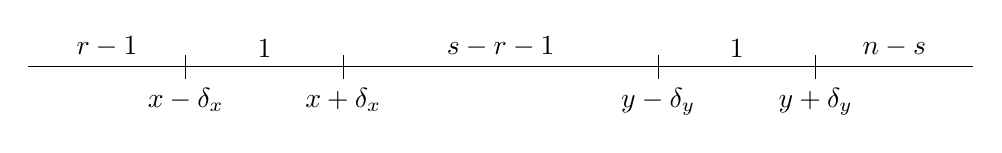
\begin{tikzpicture}
\draw(-6,0)--(6,0)
(2,0.15)--(2,-0.15)
(-2,0.15)--(-2,-0.15)
(0,0)node[above]{$s - r - 1$}
(2,-0.15)node[below]{$y - \delta_y$}
(-2,-0.15)node[below]{$x+\delta_x$}
(-4,0.15)--(-4,-0.15)
(4,0.15)--(4,-0.15)
(-4,-0.15)node[below]{$x - \delta_x$}
(4,-0.15)node[below]{$y + \delta_y$}
(5,0)node[above]{$n - s$}
(-5,0)node[above]{$r - 1$}
(-3,0)node[above]{$1$}
(3,0)node[above]{$1$};
\end{tikzpicture}
\end{figure}
$$P^n_{r-1, s-r-1, n-s} = \frac{n!}{(r - 1)!\, (s - r - 1)!\, (n - s)!}$$

$$f_{r, s}(x,y) = \frac{n!}{(r - 1)!\, (s - r - 1)!\, (n - s)!}\, \left[P(x)\right]^{r - 1}\, p(x)\, \left[P(y) - P(x)\right]^{s - r - 1}\, \left[1 - P(y)\right]^{n - s}\, p(y).$$
The joint probability function for the $r^{\text{th}}$ and $s^{\text{th}}$ order statistics with $r < s$
$$f_{r,s}(x,y) = \frac{n!\,p(x)\, p(y)}{(r - 1)!\, (s - r - 1)!\, (n - s)!}\, \left[P(x)\right]^{r - 1}\, \left[P(y) - P(x)\right]^{s - r - 1}\, \left[1 - P(y)\right]^{n - s}\hspace{0.3cm} \cdots\hspace{0.3cm}1.4.1(a)$$
If $\, r = 1, \, \, n = s\hspace{0.5cm} f_{1, n}(x, y)  = n\, (n - 1)\, p(x)\, p(y)\, \left[P(y) - P(x)\right]^{n  - 2}\hspace{0.5cm}\cdots\hspace{0.3cm} 1.4.1(b)$\\

we can also write the joint pdf of $X_{n_1}, \, X_{n_2}, \, \cdots\, , \, X_{n_k}$ where $1\leq n_1 < n_2 <\, \cdots\, < n_k\leq n$
\begin{figure}[H]
\centering
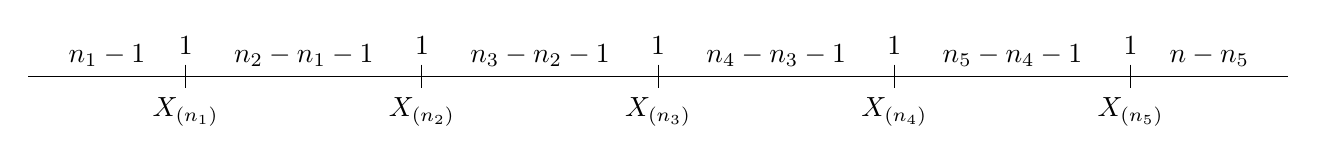
\begin{tikzpicture}
\draw(-8,0)--(8,0)
(0,0.15)--(0,-0.15)
(-3,0.15)--(-3,-0.15)
(3,0.15)--(3,-0.15)
(-6,0.15)--(-6,-0.15)
(6,0.15)--(6,-0.15)
(-7,0)node[above]{$n_1 - 1$}
(-6,-0.15)node[below]{$X_{(n_1)}$}
(-6,0.15)node[above]{1}
(-4.5,0)node[above]{$n_2 - n_1 - 1$}
(-3,-0.15)node[below]{$X_{(n_2)}$}
(-3,0.15)node[above]{1}
(-1.5,0)node[above]{$n_3 - n_2 - 1$}
(0,-0.15)node[below]{$X_{(n_3)}$}
(0,0.15)node[above]{1}
(1.5,0)node[above]{$n_4 - n_3 - 1$}
(3,0.15)node[above]{1}
(3,-0.15)node[below]{$X_{(n_4)}$}
(4.5,0)node[above]{$n_5-n_4-1$}
(6,0.15)node[above]{1}
(6,-0.15)node[below]{$X_{(n_5)}$}
(7,0)node[above]{$n - n_5$};
\end{tikzpicture}
\end{figure}


\begin{align*}
f_{X_{(n_1)}\, \cdots\, X_{(n_5)}}(x_1, \, \cdots\, , x_5)  = &  \frac{n!}{(n_1 - 1)!\, (n_2- n_1-1)!\, (n_3-n_2-1)!\,\cdots\, (n-n_5)!}\\
= & \times\, p(x_1)\, p(x_2)\, \cdots\, p(x_5)\times \left[P(x_1)\right]^{n_1 - 1}\, \left[P(x_2) - P(x_1)\right]^{n_2-n_1-1}\\
 & \times \left[P(x_3) - P(x_2)\right]^{n_3 - n_2 - 1}\, \cdots\, \left[1 - P(x_5)\right]^{n - n_5}.
\end{align*}

In general
\begin{align*}
f_{n_1, n_2, \, \cdots\, , \, n_k}(x_{n_1}, \, x_{n_2}, \, \cdots\, , \, x_{n_k}) = &  \frac{n!\,p(x_{n_1})\, p(x_{n_2})\, \cdots\, p(x_{n_k })\, \times\, \left[P(x_{n_1})\right]^{n_1 - 1}\, }{(n_1 - 1)!\, (n_2-n_1-1)!\, \cdots\, (n_k-n_{k -1}-1)!\, (n-n_k)!}\\
 & \times\,\left[P(x_{n_2}) - P(x_{n_1})\right]^{n_2 - n_1 - 1}\, \left[P(x_{n_3}) - P(x_{n_2})\right]^{n_3-n_2-1}\, \cdots\cdots\\
 & \times \, \left[P(x_{n_k}) - P(x_{n_k - n_1})\right]^{n_k - n_k-1}\, \left[1 - P(x_{n_k})\right]^{n -k}\hspace{1.5cm}  1.4.2
\end{align*}



\begin{note}
From 1.4.1 we can get the joint cdf $F_{r, s}(x,y)$ for $X_{(r)}$ and $X_{(s)}$ by integration
\end{note}
$$F_{r,s}(x,y) = \int^y_{x}\int_{-\infty}^yf_{r,s}(u,v)\, du\, dv$$ 
or we can do it by the following reasoning
\begin{align*}
F_{r,s}(x,y) & = P(X_{(r)} \leq x\, , \, X_{(s)} \leq y)\\
& = Pro\left(\text{atleast}\, \hspace{0.2cm}r \hspace{0.2cm} \text{of}\, X_i\, 's\leq x\, , \, \text{at least}\, s \, \text{of}\, X_j \,' s\leq y\right)\\
& = \sum_{j = s}^n\sum^j_{i = r}\frac{n!}{i!\, (j - k)!\, (n - j)!} \times\left[P(x)\right]^i\, \left[P(y) - P(x)\right]^{j - i}\, \left[1 - P(y)\right]^{n - j}\hspace{0.3cm} \cdots\hspace{0.3cm}1.4.3 (a)
\end{align*}

If $\, r = 1, \, s = n$
\begin{align*}
F_{1,n}(x,y) & = \sum_{j = n}^n\sum^j_{i = 1}\frac{n!}{i!\, (j - i)!\, (n-j)!}\, \left[P(x)\right]^{i}\, \left[P(y) - P(x)\right]^{j-i}\left[1 - P(y)\right]^{n - j}\\
& = \sum^n_{i = 1}\frac{n!}{i!\, (n - i)!}\, \left[P(x)\right]^i\, \left[P(y) - P(x)\right]^{n - i}\, \left[1 - P(y)\right]^{n - n}\\
& = \sum^n_{i = 1}\binom{n}{i}\, \left[P(x)\right]^{i}\, \left[P(y) - P(x)\right]^{n - i}\\
\therefore\hspace{0.3cm} F_{1,n}(x,y) & = \left(P(y)\right)^n - \left(P(y) - P(x)\right)^n \hspace{0.5cm}\cdots\cdots\hspace{0.3cm} 1.4.3 (b)\\
\end{align*}



\begin{exa}
Let $X_1, \, X_2, \, \cdots\, \, X_n$ be a random sample from exponential $p(x) = \lambda\, e^{-\lambda x},$\\ $\, \, P(x) = 1 - e^{-\lambda x}$. Find the following
\begin{enumerate}
\item[(i)] cdf for $X_{(r)}$ and also for $r = 1$, and find $r = n$.
\begin{proof}[Solution]
From equation 1.3.4
$$F_r(y)  = \frac{1}{B(r, n- r + 1)} \int_0^{1 - e^{-\lambda\, y}}t^{r - 1}\, (1 - t)^{n - r}\, dt.$$
\begin{align*}
r  = 1, \, \hspace{0.2cm} F_1(y) & = \frac{1}{B(1, n)} \int_0^{1 - e^{-\lambda\, y}} (1 - t)^{n - r}\, dt\\
 &  =  \frac{\Gamma(n + 1)}{\Gamma(1)\, \Gamma(n)}\cdot\frac{-(1 - t)^{n}}{n}\Bigg|^{1 - e^{-\lambda y}}_0\\
 & = 1 - \left(1 - 1 + e^{-\lambda y}\right)^n
\end{align*}
$F_1(y) = 1 - e^{-\lambda n y},$ cdf of the minimum, $y > 0$.

\begin{align*}
F_n(y)  = \frac{1}{B(n,1)}\int_0^{1 - e^{-\lambda y}}t^{n - 1}\, dt
 = \frac{\Gamma(n + 1)}{\Gamma(n)\, \Gamma(1)}\cdot\frac{t^n}{n}\Bigg|^{1 - e^{-\lambda n y}}_0
 = \left(1 - e^{-\lambda y}\right)^n
\end{align*}
\begin{align*}
f_n(y) & = n\, \left(1 - e^{-\lambda y}\right)^{n - 1}\, \left(-e^{-\lambda y}\right)\left(-\lambda\right)\\
& = \lambda n e^{-\lambda y}\, \left(1 - e^{-\lambda y}\right)^{n - 1}\hspace{0.3cm} y > 0.
\end{align*}
\end{proof}


\item[(ii)] joint pdf for $X_{(r)}$ and $X_{(s)}, \, r < s$ also for $r = 1$ and $s = n$.
\begin{proof}[Solution]
\begin{align*}
f_{r,s}(x,y) & = \frac{n!\, p(x)\, p(y)}{(r - 1)!\, (s-r-1)!\, (n - s)!}\left[P(x)\right]^{r - 1}\, \left[P(y) - P(x)\right]^{s - r - 1}\, \left[1 - P(y)\right]^{n - s}\\
& = \frac{n!\, \lambda^2e^{-\lambda (x + y)}}{(r - 1)!\, (s - r - 1)!\, (n - s)!}\left(1 - e^{-\lambda x}\right)^{r - 1}\, \left(e^{-\lambda} - e^{-\lambda y}\right)^{s - r - 1}\, \left(e^{-\lambda y}\right)^{n - s}\\
& = \frac{n!\, \lambda^2\, e^{-\lambda (x + y + y(n - s))}}{(r - 1)!\, (s - r - 1)!\, (n - s)!}\left(1 - e^{-\lambda x}\right)^{r - 1}\, \left(e^{-\lambda x} - e^{-\lambda y}\right)^{s - r - 1}.
\end{align*}
$r = 1, \, \, s = n$
$$f_{1,n}(x,y) = n(n - 1)\lambda^2\, e^{-\lambda (x + y)}\left(e^{-\lambda x} - e^{-\lambda y}\right)^{n - 2}\, , \hspace{0.3cm} 0 < x < y < \infty.$$
\end{proof}


\item[(iii)] joint cdf for $X_{(r)}$ and $X_{(s)}, \, r < s$ also for $r = 1$ and $s = n$.
\begin{proof}[Solution]
\begin{align*}
F_{r, s}(x,y) &  = \sum^n_{j = s}\sum^j_{i = r}\frac{n!}{i!\, (j- i)!\, (n - j)!}\left[P(x)\right]^i\left[P(y) - P(x)\right]^{j - i}\, \left[1 - P(y)\right]^{n - j}\\
& = \sum^n_{j = s}\sum^j_{i = r}\frac{n!}{i!\, (j - i)!\, (n - j)!}\left[1 - e^{-\lambda x}\right]^i\, \left[e^{-\lambda x} - e^{-\lambda y}\right]^{j - i}\left[e^{-\lambda y}\right]^{n -j}.
\end{align*}
$r = 1, \, \, s = n$
\begin{align*}
F_{1,n}(x,y) & = \sum^n_{i = 1}\frac{n!}{i!\, (n - i)!\, (n - n)!}\left[1 - e^{-\lambda x}\right]^{i}\, \left[e^{-\lambda x} - e^{-\lambda y}\right]^{n - i}\\
& = \sum^n_{i = 1}\binom{n}{i}\left[1 - e^{-\lambda x}\right]^i\, \left[e^{-\lambda x} - e^{-\lambda y}\right]^{n - i}\\
& = \left[1 - e^{-\lambda x} + e^{-\lambda x} - e^{-\lambda y}\right]^n - \left[e^{-\lambda x} - e^{-\lambda y}\right]^n\\
F_{1,n}(x,y) & = \left[1 - e^{-\lambda y}\right]^n - \left[e^{-\lambda x} - e^{-\lambda y}\right]^n.
\end{align*}
\begin{align*}
\frac{\partial}{\partial x}F_{1, n}(x,y)  & = n \lambda e^{-\lambda x}\left(e^{-\lambda x} - e^{-\lambda y}\right)^{n - 1}\\\\
\frac{\partial^2}{\partial y \, \partial x}F_{1,n}(x,y) & = n(n - 1)\lambda^2\, e^{-\lambda(x + y)}\left[e^{-\lambda x} - e^{-\lambda y}\right]^{n - 2}.
\end{align*}
\end{proof}
\end{enumerate}
\end{exa}




\section{Distribution of the Range}
The range $R = X_{(n)} - X_{(r)} > 0$ $$\left(X_{(n)}\, , \, X_{(1)}\right)\longrightarrow\, \left(R\, , \, U\right)$$
where $R = X_{(n)} - X_{(1)}, \hspace{0.2cm} U = X_{(1)}$. Hence $X_{(1)} = U, \, \, X_{(n)}  = R + U$
$$f_{1, n}(x,y) = n\, (n - 1)\, p(x) \, p(y)\, \left(P(y) - P(x)\right)^{n - 2}.$$
$$J = \begin{vmatrix}
\dfrac{\partial X_{(n)}}{\partial R} & \dfrac{\partial X_{(n)}}{\partial U}\\\\
\dfrac{\partial X_{(1)}}{\partial R} & \dfrac{\partial X_{(1)}}{\partial U}\\
\end{vmatrix} 
 = \begin{vmatrix}
 1 & 1 \\
 0 & 1\\
 \end{vmatrix} = 1.$$
\begin{align*}
f_{R,U}(r,u) & = n\, (n - 1)\, p(u)\, p(r + u)\, \left[P(r + u)  - P(u)\right]^{n - 2}\, \begin{vmatrix}
J\\
\end{vmatrix}\\
& = n\, (n - 1)\, p(u)\, p(r + u)\, \left[P(r + u) - P(u)\right]^{n - 2}.
\end{align*}
Therefore
$$f_R(r) = n\, (n - 1)\, \int_{u}p(u)\, p(r  + u)\, \left[P(r + u) - P(u)\right]^{n - 2}\, du\hspace{0.5cm}\cdots\hspace{0.3cm} 1.5.1$$


\begin{exa}
Find the pdf of the range given a random of size $n$ from exponential with mean $\frac{1}{\lambda}$
\end{exa}
\begin{proof}[\textbf{Solution.}]
\begin{align*}
f_R(r) & = n\, (n - 1)\, \int_{0}^{\infty}\lambda\, e^{-\lambda \, u}\, \lambda\, e^{-\lambda (u + r)}\, \left(1 - e^{-\lambda(u + r)} - 1 + e^{-\lambda u}\right)^{n - 2}\, du\\
&  = \lambda^2 n (n-1) e^{-\lambda r}\int_0^{\infty}e^{-2\lambda u}\left(e^{-\lambda u}\right)^{n - 2}\, \left(1  - e^{-\lambda r}\right)^{n - 2}\, du\\
& = \lambda^2\, n\, (n - 1)\, e^{-\lambda r}\, \left(1 - e^{-\lambda r}\right)^{n - 2}\int^{\infty}_0e^{-\lambda n u}\, du\\
& = n\, (n - 1)\, \lambda^2\, e^{-\lambda r}\, \left(1 - e^{-\lambda r}\right)^{n - 2}\Big[\frac{e^{-\lambda n u}}{n\lambda}\Big|_0^{\infty}\\
& = (n - 1)\, \lambda\, e^{-\lambda r}\, \left(1 - e^{-\lambda r}\right)^{n - 2}, \hspace{0.3cm} r >0.
\end{align*}
$F_r(r) = \left(1 - e^{-\lambda r}\right)^{n - 1}, \hspace{0.3cm} r \in (-\infty, \infty)$ (cdf or exponential)
\end{proof}






\section{Conditional Distribution of Order Statistic}
$X_{(r)}$ and $X_{(s)}$
$$f_r(x) = \frac{n!}{(r -1)!\, (n - r)!}\left(P(x)\right)^{r - 1}\, \left(1  - P(x)\right)^{n  - r}\hspace{0.6cm}\cdots\hspace{0.3cm}1.7.1$$
$$f_{r,s}(x,y)  = \frac{n!\, p(x)\, p(y)}{(r - 1)!\, (s  - r - 1)!\, (n - s)!}\left[P(x)\right]^{r - 1}\, \left[P(y) - P(x)\right]^{s - r - 1}\, \left[1 - P(y)\right]^{n - s}\hspace{0.3cm}\cdots\hspace{0.3cm}1.7.2$$
we want conditional distribution of $s$ given $r$

$$f_{X_{(s)}/X_{(r)}}(y/x) = \frac{f_{r,s}(x,y)}{f_r(x)}
 = \frac{(n - r)!\, p(y)\, \left(P(y) - P(x)\right)^{s - r - 1}\, \left(1 - P(y)\right)^{n - s}}{(s - r - 1)!\, (n - s)!\, \, \left(1 - P(x)\right)^{n - r}}.$$

$$f_{s/r}(y/x) = \frac{(n - r)!\, p(y)\, \left(P(y) - P(x)\right)^{s - r - 1}\, \left(1 - P(y)\right)^{n - s}}{(s - r - 1)!\, (n - s)!\, \, \left(1 - P(x)\right)^{n - r}}\hspace{0.6cm}\cdots\cdots\hspace{0.5cm} 1.7.3$$

for $s = n, \, \, r = 1$
$$f_{n/1}(y/x) = \frac{(n - 1)\, p(y)\ \left(P(y) - P(x)\right)^{n - 2}}{\left(1 - P(x)\right)^{n - 1}}.$$

Exponential
\begin{align*}
f_{n/1}(y/x) & = \frac{(n - 1)\, \lambda \, e^{-\lambda y}\, \left(e^{-\lambda x} - e^{-\lambda y}\right)^{n - 2}}{\left(e^{-\lambda x}\right)^{n - 1}}\\
& = (n - 1)\, \lambda\, e^{\lambda x (n - 1)}\, e^{-\lambda y}\, \left(e^{-\lambda x}  - e^{-\lambda y}\right)^{n - 2}, \hspace{0.3cm} y > x.
\end{align*}
 * prove that this is a pdf (Bonafide).\\
 
The result of 1.7.3 can be stated as follows.

\begin{thm}
For a random sample of size $n$ from a continuous distribution, the conditional $X_{(r)} = x \, (r < s)$ is just the distribution of the $(s - r)^{\text{th}}$ order statistic in a random sample of size $n - r$ drawn from $\frac{P(y)}{1 - P(x)}, \, y\geq x$.  The joint pdf of $X_{(n_1)}, \, X_{(n_2)}, \, \cdots\, ,\, X_{(n_k)}$ is given by $n_1< n_2,< \cdots < n_k$.
\begin{align*}
f_{n_1, n_2, \cdots\ n_k}(x_1, \, x_2, \, \cdots\, , \,x_k) = & \frac{n!\,\, p(x_1)\, p(x_2)\,\, \cdots\,\, p(x_k)}{(n_1 -1)!\, (n_2 - n_1 - 1)!\, (n_3- n_2 - 1)!\cdots (n_k - n_{k - 1} - 1)!\, (n - n_k)!}\\
& \times \left(P(x_1)\right)^{n_1 - 1}\, \left(P(x_2) - P(x_1)\right)^{n_2 - n_1 - 1}\, \cdots\, \left(P(x_k) - P(x_{k - 1}\right)^{n_k - n_{k - 1} - 1}\\
& \times \, \left(1 - P(x_k)\right)^{n - n_k}
\end{align*}
\end{thm}
It can be verified that 
$$f_{X_{(s)}/X_{(1)} = x_{r_1}, \, X_{(r - 1)} = x_{r - 1}\, \cdots\, X_{(1)} = x_1}(y) = f_{X_{(s)}/X_{(r)} = x_r}(y)$$ 
which establishes that order statistics in a random sample from a continuous distribution for a Markov chain.\\
(Use mathematical induction).\\


Now let $Z_{(1)} \leq Z_{(2)} \leq \, \cdots\, \leq Z_{(n)}$ denote the order statistics from a random sample of size $n$ from exponential with mean 1. $$p(z) = e^{-z}$$
write the joint pdf of $Z_{(1)}, \, Z_{(2)}, \, \cdots\, , \, Z_{(n)}$.
$$f_{1,2, \cdots\, n}(z_{(1)},\, z_{(2)}, \, \cdots\, , \, z_{(n)}) = n!\, e^{-z_{(1)} - z_{(2)} - --- z_{(n)}}$$
which can be written as 
$$f_{1,2, \cdots\, n}(z_{(1)},\, z_{(2)}, \, \cdots\, , \, z_{(n)}) = n!\, e^{-\sum^n_{j = 1} \left(n - j + 1\right)\left(z_{(j)} - z_{(j - 1)}\right)}, \hspace{0.3cm}\text{where}\hspace{0.3cm} z_{(0)} = 0.$$
making a transformation
$$Y_j = \left(n - j + 1\right)\left(Z_{(j)} - Z_{(j - 1)}\right),\hspace{0.3cm} j = 1, 2,\, \cdots\, , n\hspace{1cm}\cdots\hspace{0.5cm} 1.7.6$$
$$P(Y_j) = e^{-y_j}\hspace{1cm} \cdots\cdots\hspace{1cm} 1.7.7$$

We see that the $Y_j\, '$s are independent and each $Y_j$ is exponential with mean 1.\\
The relation 1.7.6 allows  $Z_{(r)}, \, r = 1, \, 2, \, \cdots\, n$ to be expressed as 
$$Z_{(r)} = \sum^r_{j = 1} \frac{Y_j}{n - j + 1}\hspace{1cm} \cdots\cdots\hspace{1cm} 1.7.8.$$
i.e as a linear function of independent random variables. It follows that $Z_{(1)}, \, Z_{(2)}, \, \cdots\, , \, Z_{(n)}$ form an additive Markov chain.\\
Equations 1.7.6, 1.7. 7 and 1.7.8 have important applications in life testing. Apart from the scale factor the $Z_{(j)}\,$'s can be interpreted as the successive failure lifetimes, of $n$ items the individual lifetime $X = \lambda Z\, (\lambda > 0)$ mean $\lambda$. The intervals of length $X_{(j)} - X_{(j - 1)}$ between successive failures are then independently distributed as $\frac{\lambda z}{ h - j + 1}$.




\section{Expected values and Moments of Order Statistics}
Let $X_1, \, X_2, \, \cdots\, , \, X_n$ be a random sample from a continuous distribution with cdf $P(x)$ and pdf $p(x)$. Let $f_r(x)$ be the pdf of $X_{(r)}$ ($r^{\text{th}}$ order statistics). 
$$\mu_r = E\left(X_{(r)}\right) = \int_x x\, f_r(x)\, dx\,, $$
$$f_r(x) = \frac{n!}{(r - 1)!\, (n - r)!}\, p(x)\, \left(P(x)\right)^{r - 1}\, \left(1 - P(x)\right)^{n - r}.$$
\begin{align*}
\mu_r & = \int_x \frac{n!}{(r - 1)!\, (n - r)!}p(x)\, \left(P(x)\right)^{r - 1}\, \left(1 - P(x)\right)^{n - r } \, dx\\
& = \frac{n!}{(r - 1)!\, (n - r)!}\int x\, \left(P(x)\right)\, \left(1 - P(x)\right)^{n - r}\, dP(x)\, , \hspace{0.5cm} \boxed{p(x)dx = dP(x)}\\
& = \frac{n\, (n - 1)!}{(r - 1)!\, (n - r)!}\int^{\infty}_{-\infty} x\, \left(P(x)\right)^{r - 1}\, \left(1 - P(x)\right)^{n - r}\, dP(x)\\
& = n\, \binom{n - 1}{r  - 1}\, \int^{\infty}_{-\infty} x\, \left(P(x)\right)^{r - 1}\, \left(1 - P(x)\right)^{n - r}\, dP(x)\hspace{1cm} \cdots\hspace{0.3cm} 1.8.1.
\end{align*}
Since  $0 \leq P(x) \leq 1$
$$|\mu_r| \leq n \, \binom{n - 1}{r - 1}\, \int |x|\, dP(x)\hspace{1cm} \cdots\hspace{0.3cm} 1.8.2$$
1.8.2 shows that $\mu_r$ exists provided $E(X)$ exists.\\

The converse is not necessary true i.e $\mu_r$ may exists even when $E(X)$ doesn't exist.\\

For equation 1.8.1, let $u = P(x)$, then $du = dP(x)$
$$P^{-1}(u) = P^{-1}\left(P(x)\right) = x$$
$$\mu_r = n\, \binom{n - 1}{r - 1}\int_0^1P^{-1}(u)\, u^{r - 1}\, \left(1 - u\right)^{n - r}\, du\hspace{1cm} \cdots\hspace{0.5cm} 1.8.3$$

If the mean $E(X) = \int^1_0P^{-1}(u)\, du$ doesn't exist because of singularities at $u = 0$, or $u = 1$, $\mu_r$ may never the less exist for certain values of $r$. For examples the Cauchy distribution $\mu_r$ exists unless $r = 1$ or $r = n$ 
$$p(x) = \frac{1}{\pi\left(1 + (x - \theta)^2\right)}.$$
If $E(g(x))$ exists where $g(x)$ is some function of $X$ then $E(g(X_{(r)})$ will also exist.\\

The special cases of the $g(\cdot)$ function
$$g(x) = x^k, \, E\left(X^k_{(r)}\right) = \text{the}\,  K^{\text{th}}\, \text{raw moment of}\,  X_{(r)}.$$
$$g(x) = \left(x - \mu\right)^{k}\, , \, \hspace{0.3cm} E\left(X_{(r)}^k - \mu^k_{r}\right)^k = \text{the}\, K^{\text{th}}\, \text{central moment of}\, X_{(r)}.$$
$$g(x) = e^{tx}\, , \, \hspace{0.3cm} E\left(e^{t X_{(r)}}\right) = \text{the mgf of the }\, r^{\text{th}}\, \text{order statistics}.$$

The product moments may be defined as usual
$$\mu_{rs} = E\left(X_{(r)}\, X_{(s)}\right)\hspace{1cm} \cdots\cdots\hspace{1cm} 1.8.4$$
$$\text{Covariance}\hspace{0.3cm} \sigma_{rs} = E\left[\left(X_{(r)} - \mu_r\right)\left(X_{(s)} - \mu_s\right)\right]\hspace{1cm}\cdots\cdots\hspace{1cm} 1.8.5$$
$$\text{Variance}\hspace{0.5cm} \sigma^{2}_{r} = E\left[\left(X_{(r)} - \mu_r\right)^2\right]\hspace{1cm}\cdots\cdots\hspace{1cm}1.8.6$$



\begin{exa}
Let $X$ be a uniform random variable on $(0,1)$. Find the following given a random sample of size $n$.
\begin{enumerate}
\item[(a)] mean and variance of $X_{(r)}$, 
\begin{proof}[Solution.]
$X\thicksim U(0,1)\,$ i.e $\, p(x) = 1, \hspace{0.5cm} P(x)  = x, \hspace{0.3cm} x \in (0, 1)$
\begin{align*}
\mu_r & = n \, \binom{n - 1}{n - r}\int^1_0x\cdot 1\cdot \cdot x^{r  - 1}\cdot (1 - x)^{n - r}\, dx\\
& = n\, \binom{n - 1}{n - r}\underbrace{\int^1_0x^r\, (1 - x)^{n - r}\, dx}_{B(r + 1, n - r+ 1}\\
& = \frac{n\, (n - 1)!}{(n - r)!\, (r - 1)!}\cdot\frac{r!\, (n - r)!}{(n + 1)!}\\
\implies\hspace{0.3cm} \mu_r  & = \frac{r}{n + 1}.
\end{align*}
If $r = 1, \hspace{0.3cm} \mu_1 = \dfrac{1}{n + 1}.$
$$E\left(X_{(r)}^2\right) = \frac{r\, (r + 1)}{(n + 1)\, (n + 2)}$$
Hence
\begin{align*}
\sigma^2_r & = E\left(X_{(r)}\right)^2  - \left(E(X_{(r)}\right)^2\\
& = \frac{r\, (r + 1)}{(n + 1)\, (n + 2)} - \left(\frac{r}{n + 1}\right)^2\\
& = \frac{(r^2  + r)}{(n + 1)\, (n + 2)} - \frac{r^2}{(n + 1)^2}\\
& = \frac{(n + 1)\, (r^2 + r) - r^2\, (n + 2)}{(n + 1)^2 \, (n + 2)}
 = \frac{nr^2 + nr + r^2 + r - nr^2 - 2r^2}{(n + 1)^2\, (n + 2)}\\
& = \frac{r\, (n + 1 - r)}{(n + 1)^2 \, (n + 2)}.
\end{align*}
\end{proof}

\item[(b)] product moment of $X_{(r)}$ and $X_{(s)}$,  $\, s>r$
\begin{proof}[Solution.]
\begin{align*}
\mu_{rs}  = & \iint \frac{n!\, xy\, x^{r - 1}\, (y - x)^{s - r - 1}}{(r - 1)!\, (s - r - 1)!\, (n - s)!}(1 - y)^{n -s}\, dx\, dy\\
= & \frac{n!}{(r - 1)!\, (s - r - 1)!\, (n - s)!}\int_0^1y\, (1 - y)^{n - s}\int^y_0 x^r\, (y - x)^{s - r - 1}\, dx \, dy\\
= & C\, \int^1_0y\, (1 - y)^{n - s}\, y^{s - r - 1}\, \int^y_0x^r\, \left(1 - \frac{x}{y}\right)^{s-r-1}\, dx\, dy\\
 & (\text{let}\, z = \frac{x}{y}\, \text{then}\, y\, dz = dx)\\
= & \frac{n!}{(r - 1)!\, (s - r - 1)!\, (n - s)!}\int^1_0y\, (1 - y)^{n - s}\, y^{s - 1}\, dy\, \int^1_0z^r\, (1 - z)^{s-r-1}\, dz\\
E\left(X_{(r)}X_{(s)}\right) & = \frac{r \, (s + 1)}{(n + 1)\, (n + 2)}.
\end{align*}
\end{proof}


\item[(c)] covariance of $X_{(r)}$ and $X_{(s)}$.
\begin{proof}[Solution.]
From (a) and (b)
\begin{align*}
Cov\left(X_{(r)}, X_{(s)}\right)  &  = E\left(X_{(r)}X_{(s)}\right) - E\left(X_{(r)}\right)\, E\left(X_{(s)}\right)\\
& = \frac{r\, (s + 1)}{(n + 1)(n + 2)} - \frac{r}{(n + 1)}\cdot\frac{s}{(n+1)}
= \frac{(n + 1)\, r\, (s  + 1) - (n + 2)\, rs}{(n + 1)^2(n + 2)}\\
%& = \frac{nrs + nr + rs + r - nrs - 2rs}{(n + 1)^2\, (n + 2)}\\
& = \frac{r\, (n - s + 1)}{(n + 1)^2\, (n + 2)}.
\end{align*}
\end{proof}
\end{enumerate}
\end{exa}



Let us consider the product moment for four order statistics
$1 \leq r < s < t < u \leq n$
\begin{align*}
f_{r,s,t,u}(x_1, x_2, x_3, x_4)  = & \frac{n!\, x_1^{r - 1}\, (x_2 - x_1)^{s - r - 1}\, (x_3 -x_2)^{t-s-1}\, (x_4 - x_3)^{u -t - 1}\, (1 - x_4)^{n - u}}{(r - 1)!(s - r - 1)!\, (t - s - 1)!\, (u - t - 1)!\, (n - u)!}\\
 & 0 < x_1 < x_2 < x_3 < x_4 < 1.
\end{align*}
making the following transformation
$\,(x_1,\,  x_2,\, x_3,\, x_4)\, \, \longrightarrow\, \, (y_1,\, y_2,\, y_3, \, y_4)$
$$x_1 = y_1y_2y_3y_4\, , \,\,\,  x_2 = y_2y_3y_4\, , \,\,\,  x_3 = y_3y_4\, , \,\,\, x_4 = y_4$$
$$J = y_2\, y_3^2\, y_4^3$$
\begin{align*}
f_{Y_1,Y_2,Y_3,Y_4}(y_1,y_2,y_3,y_4) & =A\, y_1^{r - 1}(1 - y_1)^{s - r - 1}\, y^{s  - 1}_2(1 - y_2)^{t - s - 1}\,y^{t - 1}_3(1 - y_3)^{u - t - 1}\, y_4^{u - 1}(1 - y_4)^{n - u}
\end{align*}
$$A = \frac{1}{B(r,s - r)}\cdot\frac{1}{B(u, n - u + 1)}$$





%%%%
\section{More on Moments}
An alternative formula for $\mu_r = E(X_{(r)})$ may be found by integrating by parts.
$$\mu_r = \int^{\infty}_{-\infty} x\, dF_r(x)\hspace{1cm} \cdots\hspace{1cm} *,$$
where $F_r(x)$ is the cdf of $X_{(r)}$.\\


\begin{note}
For any cdf $P(X)$ , the existence of $E(X)$ implies that
\end{note}
\begin{enumerate}
\item[(i)] $\lim\limits_{x \rightarrow - \infty}x\, P(x) = 0$
\item[(ii)] $\lim\limits_{x \rightarrow + \infty}x\, \left(1 - P(x)\right) = 0$.
\end{enumerate}

Therefore $\lim\limits_{x \rightarrow - \infty} x\, F_r(x)  = 0$ and $\lim\limits_{x \rightarrow + \infty}x\, \left(1 - F_r(x)\right) = 0\,$ since $\mu_r$ exists.\\

$*$ can be written as
$$\mu_r = \int^0_{-\infty}x\, dF_r(x) - \int_0^{\infty}x\, d\left(1 - F_r(x)\right)\hspace{1cm} \cdots\hspace{1cm} 1.8.1$$
integrating by parts
\begin{align*}
\mu_r & = x\, F_r(x)\Big|^0_{-\infty} - \int^0_{-\infty} F_r(x)\, dx - x(1 - F_r(x)\Big|^{\infty}_0  + \int_0^{\infty}\left(1 - F_r(x)\right)\, dx\\
& = \int^{\infty}_0 \left(1 - F_r(x)\right)\, dx - \underbrace{\int_{-\infty}^0F_r(x)\, dx}_{\text{let}\, y = -x\implies dy = -dx}\\
& = \int^{\infty}_0\left(1 - F_r(x)\right)\, dx - \int^0_{\infty}F_r(-y)\, \left(-dy\right)\\
& = \int^{\infty}_0\left(1 - F_r(x) - F_r(-x)\right)\, dx\\
\therefore\, \mu_r & = \int^{\infty}_0\left(1  - F_r(x) - F_r(-x)\right)\, dx\hspace{1cm} \cdots\hspace{1cm} 1.8.2
\end{align*}

The range $W = X_{(n)} - X_{(1)}$ we have $$E(W) = E(X_{(n)}) - E(X_{(1)}) = \mu_n - \mu_1$$
Therefore
\begin{align*}
E(W) & = \int^{\infty}_0\left(1 - F_n(x) - F_n(-x) - 1 + F_1(x) + F_1(-x)\right)\, dx\\
& = \int^{\infty}_0\left(F_1(x) - F_n(x) + F_1(-x) - F_n(-x)\right)\, dx\\
& = \int^{\infty}_0\left(F_1(x) - F_n(x)\right)\, dx + \underbrace{\int^{\infty}_0\left(F_1(-x) - F_n(-x)\right)\, dx}_{\text{let}\, y = -x\implies dy = -dx}\\
& = \int^{\infty}_0\left(F_1(x) - F_n(x)\right)\, dx + \int^{-\infty}_0\left(F_1(y)  - F_n(y)\right)\, (-dy)\\
& = \int^{\infty}_0\left(F_1(x) - F_n(x)\right)\, dx + \int^0_{-\infty}\left(F_1(y) - F_n(y)\right)\, dy\\
\therefore\, E(W) & = \int^{\infty}_{-\infty}\left(F_1(x) - F_n(x)\right)\, dx\hspace{1cm} \cdots\hspace{1cm} 1.8.3
\end{align*}


Recall that
$$ F_r(x)   = \sum^n_{j = r} \binom{n}{j}\, \left(P(x)\right)^j\, \left(1  - P(x)\right)^{n - j}.$$
\begin{align*}
F_1(x) & = \sum^n_{j  = 1} \binom{n}{j}\, \left(P(x)\right)^j\, \left(1  - P(x)\right)^{n - j} = 1 - \left(1 - P(x)\right)^{n}.\\\\
F_n(x) & = \left(P(x)\right)^n.
\end{align*}
Therefore 1.8.3 becomes
$$E(W)  = \int^{\infty}_{-\infty} 1 - \left(1 - P(x)\right)^n - \left(P(x)\right)^n\, dx\hspace{1.5cm}\cdots\hspace{1cm} 1.8.4$$


Useful checks on computation of the raw moments are provided by noting that 
$$\left(\sum_{r = 1}^nX^k_{(r)}\right)^m = \left(\sum_{r = 1}^nX^k_r\right)^m\hspace{1.5cm} \cdots \hspace{1cm} 1.8.5$$
For every $k$ and $m$.\\

If $k = 1$, and $m = 1$ then $$\sum^n_{r =1}X_{(r)} = \sum^n_{r = 1}X_r.$$
Taking expectation both sides we get $$\sum^n_{r = 1} \mu_r = n\, \mu\hspace{1.5cm} \cdots\hspace{1cm} 1.8.6$$

If $k  = 2$ and $m = 1$
$$\left(\sum^n_{r = 1} X^2_{(r)}\right) = \left(\sum^n_{r = 1}X_r\right)\hspace{0.4cm}\implies\hspace{0.5cm} \sum^n_{r = 1} X_{(r)}^2 = \sum^n_{r = 1}X_r^2.$$
Taking expectation both sides
\begin{align*}
\sum^n_{r = 1}E\left(X^2_{(r)}\right) & = \sum^n_{r = 1} E\left(X^2_r\right) = n\, (\sigma^2 + \mu^2)\\
\sum^n_{r = 1}E\left(X^2_{(r)}\right) & = n\, (\sigma^2 + \mu^2)\hspace{1.5cm} \cdots\hspace{1cm} 1.8.7
\end{align*}


If $k  = 1$, and $m = 2$
$$\left(\sum^n_{r = 1} X_{(r)}\right)^2 = \left(\sum^n_{r = 1}X_r\right)^2$$

$$\sum^n_{r = 1}X_{(r)}\cdot\sum^n_{r  = 1} X_{(r)} = \sum^n_{r = 1} X_r \, \sum^n_{r = 1} X_r$$

$$\sum^n_{i = 1}\sum^n_{j = 1} X_{(i)}\, X_{(j)} = \sum^n_{i = r}\sum^n_{j = 1}X_i\, X_j$$

$$\sum^n_{i = 1} X_{(i)}^2 + 2\underset{i < j}{\sum\sum} X_{(i)} \, X_{(j)} = \sum^n_{i = 1} X_i^2 + 2\underset{i<j}{\sum\sum}X_i\, X_j$$
Taking expectations both sides we get
\begin{align*}
\sum^n_{i = 1} E\left(X^2_{(i)}\right)  + 2\, \underset{i< j}{\sum\sum}E\left(X_{(i)}\, X_{(j)}\right) & = n(\sigma^2 + \mu^2) + 2\, \binom{n}{2}\, \mu^2\\
&  = n\sigma^2 + n\mu^2 + n(n - 1)\mu^2\\
& = n\sigma^2 + n\mu^2 + n^2\mu^2 - n\mu^2\\
& = n\sigma^2 + n^2\sigma^2\\
& = n(\sigma^2 + n\mu^2).
\end{align*}


$$\sum^n_{r = 1} E\left(X_{(i)}^2\right) + 2\, \underset{r<s}{\sum\sum}E\left(X_{(r)}\, X_{(s)}\right)\hspace{1.5cm} \cdots\hspace{1cm} 1.8.8$$

$$\sum^n_{r = 1} X_{(r)} = \sum^n_{r = 1} X_{(r)}$$

$$\sum^n_{r = 1} \left(X_{(r)} - \mu_r\right) = \sum^n_{r = 1} (X_r   - \mu)$$
squaring both sides
$$\sum^n_{r = 1}\sum^n_{s = 1}\left(X_{(r)} - \mu_r\right)\,\left(X_{(s)} - \mu_s\right) = \sum^n_{r = 1}\sum^n_{s = 1}\left(X_r - \mu\right)\, \left(X_s - \mu\right).$$

Taking expectation both sides
$$\sum^n_{r  =1}\sum^{n}_{s = 1}Cov\left(X_{(r)},X_{(s)}\right) = \sum^n_{r = 1}\sum^n_{s = 1} Cov\left(X_r, X_s\right)$$

$$\sum^n_{r = 1}\sigma^2_r + 2\, \underset{r<s}{\sum\sum}Cov\left(X_{(r)}, X_{(s)}\right) = n\sigma^2\hspace{1.5cm} \cdots\hspace{1cm}1.8.9$$ (This is true for any distribution)\\

Read!!! Discrete case of order statistics.\\


\begin{exa}
Let $X_1, \, X_2, \, \cdots\, , \, X_n$ be random sample from exponential with mean $1/\lambda$.
$$P(x) = 1 - e^{-\lambda\, x}$$

$$E(W)  = \int^{\infty}_{-\infty}\left(1 - \left(1 - P(x)\right)^n - \left(P(x)\right)^n\right)\, dx$$

$$E(W) = \int^{\infty}_01 - e^{-\lambda nx} - \left(1 - e^{-\lambda x}\right)^n\, dx$$
Let $u = 1 - e^{-\lambda x} \,\, \implies\, \, du = \lambda e^{-\lambda x}\, dx$
$$e^{-\lambda x} = 1 - u\hspace{1cm} \frac{du}{\lambda (1 - u)} = dx$$
\begin{align*}
E(W) & = \int^1_0 1 - (1 - u)^n - u^n \, \frac{du}{\lambda (1 - u)}\\
& = \frac{1}{\lambda}\int^1_0-(1 - \mu)^{n - 1}\, du + \frac{1}{\lambda}\int^1_0\frac{1 - u^n}{1 - u}\, du\\
& = \frac{1}{\lambda}\cdot\frac{(1 - u)^n}{n}\Big|^1_0 + \frac{1}{\lambda}\int^1_0\sum_{k = 0}^{n - 1} u^k\, du\\
& = \frac{1}{\lambda n} + \frac{1}{\lambda}\sum^{n - 1}_{k = 0}\frac{u^{k + 1}}{k + 1}\Big|^1_0\\
& = \frac{1}{\lambda n} + \frac{1}{\lambda}\sum^{n - 1}_{k  = 0}\frac{1}{k + 1}.
\end{align*}
\end{exa}

















%-------------------------------------------------------------------------------------------------------------------------------------------

\chapter{DISTRIBUTION-FREE STATISTIC}
\section{Distribution-Free Statistic over a $\mathscr{Z}$} 
Let $V_1, V_2, \cdots, V_n$ be random variables with a joint distribution denoted by $D$ where $D$ is member of $\mathscr{Z}$ class of possible joint distribution. Let $T(V_1, V_2, \cdots V_n)$ denote some statistic based on $V_1, V_2, \cdots , V_n.$

\begin{defn}
 The statistic $T(V_1, V_2, \cdots, V_n)$ is said to be distribution-free over $\mathscr{Z}$ if the distribution of $T(V_1, V_2, \cdots, V_n)$ is the same for every joint distribution in $\mathscr{Z}$.
\end{defn}

\begin{enumerate}
\item[(i)] Let $\mathscr{Z}_1$ denote the collection of joint distributions on $n\, iid\, N(\mu_0, \sigma^2)$, $\, \mu_0$ is known while $\sigma^2$ is unknown.\\

$D\in \mathscr{Z}_1\, \longrightarrow\, D$ has joint of $n$-normal with mean $\mu_0, \, \sigma^2$.\\

Let $V_1, V_2, \cdots, V_n$ be a random sample from $N(\mu_0, \sigma^2)$.\\

Let $\overline{V} = \dfrac{1}{n}\sum^n_i V_{i=1}\hspace{0.3cm}$ and $\, S^2 = \dfrac{1}{n - 1} \sum^n_{i = 1} (V_i - \overline{V})^2$ sample mean and sample variance.\\

Let $U_1 = \dfrac{\sqrt{n}\, (\overline{V} - \mu_0)}{S}\,$ and $\, U_2 = \frac{(n-1)\, S^2}{\sigma^2_0}$
$$U_1 = \frac{\sqrt{n}\,\, (\overline{V} - \mu_0)}{S} \, \thicksim \, t_{n-1}$$
for whatever value of $\sigma^2$.\\
$U_1$ is distribution-free over $\mathscr{Z}_1$.


\item[(ii)] Let $\mathscr{Z}_2$ denote a collection of joint distribution of $n\,  iid \, N(\mu, \sigma^2_0)$, $\, \sigma^2_0$ is known. Let 
$$U_2 = \frac{(n-1)\, S^2}{\sigma^2_0}\, \thicksim\, \chi^2_{n-1}$$
$U_2$ is distribution-free over $\mathscr{Z}_2$. 
\end{enumerate}


\begin{defn}
Two random variables $T_1$ and $T_2$ are said to be equal in distribution denoted by $T_1\overset{d}{=}T_2$  if they have the same cdf (applies to vectors, i.e we talk of joint pdf).
\end{defn}
 
 
 \newpage
\begin{remark}
\begin{enumerate}
\item[(i)] $\overset{d}{=}$ is read as ``has the distribution as"
\item[(ii)] $X \overset{d}{=} X$
\item[(iii)] If $\, X\overset{d}{=} Y\, \implies\, Y \overset{d}{=} X$
\item[(iv)] If $X \overset{d}{=} Y\,$ and $\, Y\overset{d}{=}Z\, \implies\, X\overset{d}{=} Z$.\\
\end{enumerate}
\end{remark}


\begin{thm}
A random variable $X$ has a distribution that is symmetric about $\beta$ if and only if $X- \beta \overset{d}{=}\beta - X$.
\end{thm}
 
 
 
\begin{proof}
Suppose $X$ is symmetrical about $\beta$, we show that $X - \beta \overset{d}{=} \beta - X$.\\
Let $F(\cdot)$ denote the cdf of $X$, then 
$F_X(\beta + t) = 1 - F\left((\beta - t)^-\right) \hspace{0.3cm} \forall t\in \mathbb{R}\hspace{0.3cm}\cdots\hspace{0.3cm} (*)$.\\
The cdf of $W = X  - \beta$, 
$$G(w) = P(W\leq w) = P(X-\beta \leq w) = P(X\leq w +\beta ) = F(w + \beta)$$
the cdf of $U = \beta - X$, 
$$H(w) = P(U\leq w) = P(\beta  - X \leq w) = 1  - P(X\leq \beta - w) = 1 - F(\beta - w).$$
cdf of $X - \beta = F(w + \beta)\,$ and cdf of $\, \beta - X = 1 - F(\beta - w)$.\\

From $(*)$ we have $F(w  + \beta) = 1 - F(\beta - w)$
$$\implies\hspace{0.4cm} X - \beta \overset{d}{=} \beta - X$$
Conversely, we show that if $X- \beta \overset{d}{=} \beta - X$ then $X$ is symmetric about $\beta$.
\begin{align*}
F_X(\beta + t) & = P(X\leq \beta + t) = P(X - \beta \leq t)\\
& = P(\beta - X \leq t ) = P(\beta - t \leq X)\\
& = 1 - P(X\leq \beta - t)\\
F_X(\beta + t) & = 1 - F(\beta - t)
\end{align*} 
$\implies\hspace{0.3cm} X$ is symmetric about $\beta$.
\end{proof}





\newpage
\begin{remark}
\begin{enumerate}
\item[(i)] If a random variable $Y$ has a cdf of the form $F(Y - \theta)$, then $\theta$ is known as the location parameter. Therefore if $X$ has cdf $F(t)$ and $Y$ has cdf of $F(t - \theta)$ then $X\overset{d}{=} Y - \theta$.
\item[(ii)] If a random variable $Y$ has a cdf of the form $F(t/\eta) \,\hspace{0.2cm} \forall \, 0 < \eta < \infty$, then $Y$ is said to have a distribution indexed by the sample parameter $\eta$. Thus is $X$ has cdf of the form $F(t)$ and $Y$ has cdf of the form $F(t/\eta)$ then $X\overset{d}{=}Y/\eta$.\\
\end{enumerate}
\end{remark}



\begin{exa}
Let $X_{(1)}, X_{(2)}, \cdots, X_{(n)}$ denote the order statistics for a random sample of size $n$ from normal distribution with mean zero and variance $\sigma^2\hspace{0.3cm} (0 < \sigma^2 < \infty)$ unknown.\\
Consider the statistic $Q$ defined by 
$$Q = \frac{(X_{(n)} + X_{(1)})/2}{X_{(n)} - X_{(1)}}$$
If $Z_1, \, Z_2, \, \cdots,\, Z_n$ are $iid\, \, N(0, 1)$
$$Z_1, \, Z_2, \, \cdots, \, Z_n \, \overset{d}{=}\, \frac{X_1}{\sigma}\, , \, \frac{X_2}{\sigma}\, ,\, \cdots\, \, \, \frac{X_n}{\sigma}$$
$$Z_{(1)}, \, Z_{(2)}, \, \cdots, \, Z_{(n)}\,  \overset{d}{=}\,  \frac{X_{(1)}}{\sigma}\, , \, \frac{X_{(2)}}{\sigma}\, ,\, \cdots\, \, \, \frac{X_{(n)}}{\sigma}$$
\begin{align*}
\frac{(X_{(n)}/\sigma \, + \, X_{(1)}/\sigma)/2}{X_{(n)}/\sigma\, - \, X_{(1)}/\sigma} & \overset{d}{=}\, \frac{(Z_{(n)} + Z_{(1)})/2}{Z_{(n)} - Z_{(1)}}\\\\
& \overset{d}{=} \frac{(X_{(n)} + X_{(1)})/2}{X_{(2)} - X_{(1)}}\\\\ & = \, Q
\end{align*}
Thus for $\sigma^2 > 0$, the statistics $Q$ has the same distribution as if it were constructed using observations from $N(0,1)$. Therefore statistic $Q$ is distribution free over the class $\mathscr{Z}_3$ of the joint distribution of $iid\, \, N(0, \sigma^2)$.
\end{exa}



\begin{remark}
Even though statistics $U_1, \, U_2$ and $Q$ are distribution-free over the classes $\mathscr{Z}_1,\, \mathscr{Z}_2$ and $\mathscr{Z}_3$ respectively we would not typically consider them to be non-parametric statistics. This is so because their distributions are different if the underlying distribution is something other than normal distribution.
\end{remark}


\begin{defn}
A statistic $T$ is said to be non-parametric distribution-free if the class $\mathscr{Z}$ of joint distribution for which $T$ is distribution-free includes more distribution form than one.
\end{defn}
 
 
 
 
 
 \section{Counting Statistics}
 The simplest of all non-parametric distribution-free statistics are those based on counts of whether a particular event happens in each of the $n$ independent trials. Let $X_1, \, X_2, \cdots, \, X_n$ be independent random variables such that $X_i$    is continuous random variable cdf $F_i(x), \,\, \, i = 1, \, 2, \, \cdots, \, n$.\\
Let $F_i(\theta) = P(X_i < \theta) = P_0\, , \, \, 0 < P_0 < 1\,  \hspace{0.2cm} i = 1, \, 2, \, \cdots, \, n$ that is each $X_i$ has the same unknown $P_0^{\text{th}}$ percentile or Quantile.\\
Let $\theta_0$ be a known real number and define a statistic $\Psi_i$ by 
$$\Psi_i = \Psi(X_i - \theta_0) =
\begin{cases}
1 & X_i - \theta_0 > 0\\
& \iff X_i > \theta_0\\\\
0 & X_i - \theta_0 \leq 0\\
  & X_i \leq \theta_0\\
\end{cases}\hspace{0.5cm}\cdots\cdots\hspace{0.3cm} 2.2.1
$$

$$\Psi_i = 
\begin{cases}
1 & X_i > \theta_0\\
0 & X_i \leq \theta_0\\
\end{cases}
\hspace{0.5cm} i = 1,\, 2, \, \cdots, \, n$$ 
 
 
 
\begin{thm}
 Let $\Psi_1, \, \Psi_2, \, \cdots\, , \, \Psi_n$ be defined by $2.2.1$ and let $T(\Psi_1, \, \Psi_2, \, \cdots, \, \Psi_n)$ be any statistic based on $\Psi_1, \, \Psi_2, \, \cdots, \, \Psi_n$ only. Then if $\theta = \theta_0$
 \begin{enumerate}
 \item[(i)] the statistic $\Psi_1, \, \Psi_2, \, \cdots, \, \Psi_n$ are $iid$ Bernoulli with parameter $1 - P_0$.
 \item[(ii)] $T(\Psi_1, \, \Psi_2, \, \cdots, \, \Psi_n)$ is non-parametric distribution-free statistic over the class $\mathscr{Z}_4$, consisting of all joint distribution of independent continuous random variables each with $P_0^{\text{th}}$ quantile equal to $\theta_0$.
 \end{enumerate}
\end{thm}

\begin{proof}
The proof is trivial.
\end{proof}

The particular function of $\Psi_i's$ that are useful in hypothesis testing situation is 
$$T = T(\Psi_1, \, \Psi_2, \, \cdots, \, \Psi_n) = \sum^n_{i = 1} \Psi_i.$$
$T\thicksim B(n, 1 - P_0)$, provided the joint distribution is in class $\mathscr{Z}_4$. In particular when\\ $P_0 = \frac{1}{2}\, \implies\, \theta_0$ is the median.\\
$H_0: $ each $X_i \hspace{0.2cm} i = 1, \, 2, \, \cdots,\, n$ has median $\theta_0$ then $T = \sum^n_{i = 1}\Psi_i$ is known as the sign test statistic.
 
 


\section{Ranking Statistics} 
We consider another technique for constructing non-parametric distribution free statistics. Let $X_1, \, X_2, \, \cdots\, ,\, X_n$ be a random sample from a continuous distribution with cdf $F(x)$, and let $X_{(1)}, \, X_{(2)}, \cdots\,, \, X_{(n)}$ be the corresponding order statistics.
 

\begin{defn} 
The sample observation $X_i$ is said to have rank $R_i$ among $X_1, \, X_2, \, \cdots, X_n$ if $X_i = X_{R_i}$ provided the $R_i^{\text{th}}$ order statistic is uniquely defined.\\
Let $R = (R_1,\, R_2, \, \cdots, \, R_n)$ where $R_i$ is the rank of $X_i$ $\hspace{0.2cm} R$ is the vector of ranks.
\end{defn}



\begin{thm}
Let $X_1, \, X_2, \, \cdots\, , \, X_n$ be a random sample from continuous distribution and let $R = (R_1, \, R_2, \, \cdots\, , \, R_n)$  be a vector of ranks. If $\mathcal{B} = \{r:\, r$ is a permutation of integers $1,\, 2, \, \cdots,\, n\}$, then $R$ is uniformly distributed over $\mathcal{B}$.
\end{thm}

\begin{proof}
We note that there are $n!$ elements in $\mathcal{B}$. We need to show that $R$ assumes each of the permutations of $(1,\, 2,\, \cdots,\, n)$ with probability $\dfrac{1}{n!}$.\\

Let $r = (r_1, \, r_2, \, \cdots, \, r_n)$ be an arbitrary element in $\mathcal{B}$. Then
\begin{align*}
P_{pro}(R = r) & = P\left((X_1,\, X_2,\, \cdots,\, X_n) = (X_{(r_1)}, \, X_{(r_2)},\, \cdots\,,\,X_{(r_n)}\right)\\
&  = P(X_{d_1} < X_{d_2} < X_{d_3} < \cdots < X_{d_n})
\end{align*} 
where $d_i$ is the position of the number $i$ in the  permutation $r$, for $i = 1, \, 2, \, \cdots, \, n$.\\
Note that if $Y_1, \, Y_2,\, \cdots\, ,\, Y_m$ are $iid$ random variables and  $(\alpha_1, \, \alpha_2, \, \cdots\,, \, \alpha_m)$ is any permutation of the integers $(1, \, 2,\, \cdots\, , \, m)$
$$\left(Y_1, \, Y_2, \, \cdots\cdots\, , \, Y_m\right)\, \overset{d}{=}\, \left(Y_{\alpha_1}, \, Y_{\alpha_2}, \, \cdots\cdots\, , \, Y_{\alpha_m}\right)$$
Therefore $\,\left(X_1, \, X_2, \, \cdots\cdots\, , \, X_m\right)\, \overset{d}{=}\, \left(X_{d_1}, \, X_{d_2}, \, \cdots\cdots\, , \, X_{d_m}\right)\,$ which implies that $$P(X_{d_1} < X_{d_2} < X_{d_3} < \cdots < X_{d_n}) = P(X_1 < X_2 < X_3 < \cdots < X_n).$$
Thus
\begin{align*}
P(R = r) & = P(X_{d_1} < X_{d_2} < X_{d_3} < \cdots < X_{d_n})\\
 & = P(X_1 < X_2 < X_3 < \cdots < X_n)\\
& = P(R = r_0)\hspace{0.3cm}, \hspace{0.5cm}\text{where}\hspace{0.2cm} r_0 = (1, \, 2,\, \cdots\, , \, n)
\end{align*}
since there are $n!$ elements in $\mathcal{B}$, the result follows since $r$ is an arbitrary element in $\mathcal{B}$.
$$\sum_{r\in\mathcal{B}} P(R = r) = 1.\hspace{1.5cm} n!\, (a) = 1 \, \implies \, a = \frac{1}{n!}$$
\end{proof}



\begin{coro}
Let $X_1, \, X_2, \, \cdots\, , \, X_n$ be a random sample from a continuous distribution, and let $R$ be the corresponding vector of ranks, where $R_i$ is the rank of $X_i$  among the $n$ random variables
\begin{itemize}
\item[(a)]
\begin{itemize}
        \item[(i)] $P(R_i = r) = \begin{cases}
        \dfrac{1}{n} & \text{for}\hspace{0.2cm} r = 1, \, 2, \, \cdots\, , \, n\\
        0 & \text{elsewhere}
        \end{cases}$\\
        
        \item[(ii)] $P(R_i = r\, , \, R_j = s)_{i\neq j} = \begin{cases}
        \dfrac{1}{n\, (n - 1)} & \text{if}\hspace{0.2cm} r\neq s\\
        0 & \text{elsewhere}
        \end{cases}$\\
\end{itemize}

\item[(b)]
\begin{itemize}
           \item[(i)] $E(R_i) = \dfrac{n + 1}{2} \, \, , \,\, i = 1, \, 2, \, \cdots\cdots\, , \, n$
           
           \item[(ii)]$var(R_i) = \dfrac{(n + 1)(n-1)}{12}$
           
           \item[(iii)] $Cov(R_i, R_j) = \dfrac{-(n+1)}{12}\hspace{0.2cm}, \hspace{0.3cm} i \neq j.$\\
\end{itemize}
\end{itemize}
\end{coro}




\begin{coro}
Let $X_1, \, X_2,\, \cdots\, , \, X_n$ be a random sample from continuous distribution and let $R = (R_1, \, R_2, \, \cdots\, , \, R_n)$ is a vector of ranks. If $T(R)$ is a statistic based on $(X_1, \, X_2, \, \cdots\, , \, X_n)$, then $T(R)$  is distribution-free statistics, over the class $\mathscr{Z}_5$ of joint distributions of $n\,\, iid\,$ continuous univariate random variables i.e $T(R)$ is non-parametric distribution-free over $\mathscr{Z}_5$.
\end{coro}




Let $X_1, \, X_2,\, \cdots\, , \, X_m$ and $Y_1, \, Y_2,\, \cdots\, , \, Y_n$ be independent random samples from continuous distributions functions $F(x)$ and $G(x) = F(x - c)$ respectively where $-\infty < c < \infty$ known as the shift parameter. $(X_i \overset{d}{=} Y_i - c)$
\begin{table}[H]
\centering
\begin{tabular}{cl}
$H_0: \, c = 0\, $ vs $\, $ & $\,H_{a_1}:\, c < 0$\\
                            & $\,H_{a_2}: \, c > 0$\\
                            & $\,H_{a_3}:\, c\neq 0$.\\
\end{tabular}
\end{table}



Let $Q_i\, , \, \hspace{0.2cm} i = 1, \, 2, \, \cdots\, , \, m$ and $R_j\,  , \, \hspace{0.2cm} j = 1, \,  2, \, \cdots\, , \, n$ be the ranks of $X_i$ and $Y_j$ respectively, among $N = m + n$ combined $X$ and $Y$ observations. Thus the rank vector $$R = \left(Q_1, \, Q_2, \, \cdots\, , \, Q_m\, , \, R_1, \, R_2,\, \cdots\, , \, R_n\right)$$ is simply a permutation of $(1,\, 2,\, \cdots\, ,\, N)$, where $N = m + n$ and though random must satisfy
$$\sum^m_{i = 1} Q_i \, + \, \sum^n_{j = 1} R_j \, = \, \frac{(n + m)(n + m + 1)}{2}.$$
To construct a suitable critical region for testing $H_0 : c = 0$ vs $H_{a_1}:\, c> 0$ we must decide which rank vector is in support of $H_{a_1}$. Intuitively to the $X_i\,'s$. One such statistic is the sum of the ranks for the $Y_j\, 's$ proposed by Wilcoxon (1945) and studied independently by Mann and Whitney (1947). The test statistic proposed by Wilcoxon is 
\begin{equation}
W_y = \sum^n_{j = 1} R_j 
\end{equation}
thus $W_y$ is the sum of the ranks of $Y_j\, 's$ when ranked among all the $n + m$ observations. The statistic suggested by Mann and Whitney is 
\begin{equation}
U_y = \sum^m_{i = 1}\sum^n_{j = 1} \Psi(Y_j - X_i)
\end{equation}
where
$$\Psi(t) = \begin{cases}
1 & \text{if}\hspace{0.2cm} t > 0\\
0 & \text{if}\hspace{0.2cm} t\leq 0\\
\end{cases}
$$

$U_y$ represents the total number of times a $Y$ observation is larger than an $X$ observation when they are no ties among $X$ and $Y$ observation $W_y$ and $U_y$ are linearly related by 
\begin{equation}
W_y = U_y \, + \, \frac{n (n + 1)}{2}
\end{equation}




\begin{remark}
\begin{enumerate}
\item If $W_x = \sum^m_{i = 1} Q_i$ and $U_x = \sum^m_{i = 1}\sum^n_{j = 1} \Psi(X_i - Y_j)$ then $\, W_x = U_x + \dfrac{m(m + 1)}{2}$
\item The statistic $W_y$ is a function of the data only through the rank vector\\ $R = \left(Q_1, \, Q_2, \, \cdots\, , \, Q_m\, , \, R_1, \, R_2,\, \cdots\, , \, R_n\right)$. Under $H_0:\, c = 0$ observations\\ $X_1, \, X_2, \, \cdots\, , \, X_m \, , \, Y_1, \, Y_2, \, \cdots\, , \, Y_n$ are iid continuous random variables and by corollary 2.3.4 the rank statistic $W_y$ is non-parametric distribution-free.\\
\end{enumerate}
\end{remark}







\begin{thm}
Let $W_y$ be the Mann-Whitney/Wilcoxon rank sum statistics for testing $H_0:\, c = 0\, $ vs $\, H_a:\, c > 0$, when $X_1, \, X_2, \, \cdots\, , \, X_m$ and $\, Y_1, \, Y_2, \, \cdots\, , \, Y_n$ are independent random samples from $F(x)$ and $F(y - c)$, respectively. Under $H_0:\, c = 0$ the distribution of $W_y$ is given $$P_{H_0}\left(W_y = w\right) = \begin{cases}
\dfrac{t_{m,n}(w)}{\binom{N}{n}} & , \, w = \frac{n(n+1)}{2}\, , \, \frac{n(n+1)}{2} + 1,\, \cdots\,,\, \frac{n(n+1)}{2} + nm\\\\
0 & ,\,\,\text{otherwise}\\
\end{cases}$$
where $t_{m,n}(w)$ is the number of unordered subsets of $n$ integers taken (without replacement) from $\{1, \, 2, \, \cdots\, , \, N\}$ for which the sum is equal to $w, \, N = n + m$.\\
\end{thm}





\begin{exa}
For case $m = 3$ and $n  = 2$ there are $\binom{5}{2} = 10$ arrangements to be examined to obtain the distribution of $W_y$\\
%\begin{table}[H]
%\centering
\begin{minipage}{4in}
\begin{tabular}{cccccc}
\multicolumn{5}{c}{Arrangement} & Value of\\
1 & 2 & 3 & 4 & 5 & $w$\\
$x$ & $x$ & $x$ & $y$ & $y$ & 9\\
$x$ & $x$ & $y$ & $x$ & $y$ & 8\\
$x$ & $y$ & $x$ & $x$ & $y$ & 7\\
$y$ & $x$ & $x$ & $x$ & $y$ & 6\\
$x$ & $x$ & $y$ & $y$ & $x$ & 7\\
$x$ & $y$ & $x$ & $y$ & $x$ & 6\\
$x$ & $y$ & $y$ & $x$ & $x$ & 5\\
$y$ & $x$ & $y$ & $x$ & $x$ & 4\\
$y$ & $y$ & $x$ & $x$ & $x$ & 3\\
$y$ & $x$ & $x$ & $y$ & $x$ & 5\\
\end{tabular}
\end{minipage}
\hfill
\begin{minipage}{4in}
\begin{tabular}{c|c}
$w$ & $P\left(W_y = w\right)$\\
\hline
3 & $1/10$\\
4 & $1/10$\\
5 & $2/10$\\
6 & $2/10$\\
7 & $2/10$\\
8 & $1/10$\\
9 & $1/10$\\
\hline
\end{tabular}\\\\\\
$\alpha = 0.2$. Reject $H_0$ if  $W_{cal} \geq 8$
\end{minipage}
%\end{table}
\end{exa}

\vspace{0.5cm}





\begin{thm}
Let $W_y = \sum^n_{j = 1} R_j$ be the Wilcoxon rank statistic when $H_0:\, c = 0$ is true, the distribution of $W_y$ is symmetric about the value $$\mu = \frac{n(m + n + 1)}{2}.$$ Given independent random samples $X_1, \, X_2, \, \cdots\, ,\, X_m$ and $Y_1, \, Y_2, \, \cdots\, ,\, Y_n$ with rank vector $R = \left(Q_1, \, Q_2, \, \cdots\, , \, Q_m\, , \, R_1, \, R_2,\, \cdots\, , \, R_n\right)$ for combined sample.
\end{thm}


\begin{proof}
Recall that under $H_0$ the rank vector $R$ is uniformly distributed (theorem 2.3.2), the set of permutations of integers $(1,\, 2, \, \cdots\, , N)$ where $N= n + m$. We note that under $H_0: c = 0,$   $\, \left(-X_1, \,-X_2, \, \cdots\, , \, -X_m, \, -Y_1, \, -Y_2, \, \cdots\, , \, -Y_n\right)$ are $iid$ continuous random variables and so their rank vector is also uniformly distributed on $\mathcal{B}$. However multiplying by $-1$ makes the largest be the smallest and so forth, and hence the reverse the order of ranking. Therefore the rank vector of $\left(-X_1, \,-X_2, \, \cdots\, , \, -X_m, \, -Y_1, \, -Y_2, \, \cdots\, , \, -Y_n\right)$ written in terms of the components of the original $R$ is $$\left(N + 1 - Q_1, \, N + 1 - Q_2, \, \cdots\, , \, N + 1 - Q_m\, , \, N + 1 - R_1, \, N + 1 - R_2,\, \cdots\, , \, N + 1 - R_n\right).$$ Therefore
$$
\left(Q_1,\, \cdots\, , \, Q_m\, , \, R_1,\, \cdots\, , \, R_n\right) \, \overset{d}{=}\left(N + 1 - Q_1, \, \cdots\, , \, N + 1 -Q_m\, , \, N + 1 - R_1, \, \cdots\, , \,N + 1 -  R_n\right)$$
computing the rank sum statistic on each side and applying the theorem which says that  if $Z\overset{d}{=}V$ and $K(\cdot)$ a measurable function then $K(Z) \overset{d}{=} K(V)$. $$W_y = \sum^n_{j = 1} R_j \overset{d}{=} \sum^n_{j = 1} (N + 1 - R_j)$$
$$W_y \overset{d}{=} n(N+ 1) - \sum^n_{j = 1} R_j = n(N + 1) - W_y$$
$$W_y \overset{d}{=} n(N+1) - W_y$$
\begin{align*}
W_y - \frac{n(N+1)}{2}\, & \overset{d}{=}\, n(N+1)- W_y - \frac{n(N+1)}{2}\\\\
W_y - \frac{n(N+1)}{2}\, & \,\overset{d}{=} \frac{n(N+1)}{2} - W_y
\end{align*}
$\implies\hspace{0.3cm} W_y\,$ is symmetric at $\, \dfrac{n (N + 1)}{2}$.
\end{proof}




\begin{remark}
\begin{enumerate}
\item For testing $H_0:\, c = 0$ vs $H_a:\, c < 0$, we want critical region of the form. Reject $H_0$ if and only if $W_y \leq W'(\alpha, m, n)$ value where $\alpha$ is the level of significance and $W'(\alpha, m, n)$ is the value such that $$P\left(W_y \leq W'(\alpha, m, n)\right) = \alpha.$$
From the proof of theorem 2.3.7 we see that
$$W'(\alpha, m, n) = n(m + n + 1) - W(\alpha, m , n)$$
where $P\left(W_y\geq W(\alpha, m, n)\right) = \alpha$.
\item In the similar way, the critical region for testing $H_0: c =  0$ vs $H_a: c \neq 0$, reject $H_0$ at $\alpha$ level of significance if and only if $W_y \geq W(\alpha/2, m , n)$ or $\, W_y \leq W'(\alpha/2, m, n)$ or $\, W_y \leq n(n + m  + 1) - W(\alpha/2, m , n)$, or equivalently
$$\begin{vmatrix}
W_y - \dfrac{n(m + n + 1)}{2}\\
\end{vmatrix}\, \geq \, \begin{vmatrix}
W(\alpha/2, m , n) - \dfrac{n(m + n + 1)}{2}\\
\end{vmatrix}.$$
\item Theorem 2.3.7 also provides us with the mean of $W_y$ under $H_0: c = 0$
\end{enumerate}
\end{remark}



\section{Statistics Utilizing Counting and Ranking}
A third basic technique for constructing distribution-free statistics combines the two techniques considered in sections 2.2 and 2.3.\\
Let $Z_1, \, Z_2, \, \cdots\, , \, Z_n$ be a random sample from a continuous distribution that is symmetric about zero. Note that the point of symmetry could be any known value. If $X$ is symmetrically distributed about $\theta_0$, then $Z = X - \theta_0$ is symmetrically distributed at zero.


\begin{defn}
Define $\, \Psi_i = \Psi(Z_i)$, where 
$$\Psi (t) = \begin{cases}
1 & \text{if}\hspace{0.3cm} t > 0\\
0 & \text{if}\hspace{0.3cm} t \leq 0\\
\end{cases}$$
\end{defn}


\begin{lem}
Let $Z$ be a continuous random variable that is symmetric about zero, then the random variables $|Z|$ and $\Psi(Z)$ are stochasticaly independent.
\end{lem}

\begin{proof}
\begin{align*}
P\left(\Psi(Z) = 1\, , \, |Z| \leq t\right) &  = P\left(Z>0\, , \, |Z| \leq t\right)\\
& = P\left(0 < Z \leq t\right)\\
& = \frac{1}{2}\, P\left(-t \leq Z \leq t\right)\\
& = P\left(\Psi(Z) = 1\right)\, P\left(|Z|\leq t\right)\\
P\left(\Psi(Z) = 1\, , \, |Z| \leq t\right) &  = P\left(\Psi(Z) = 1\right)\, P\left(|Z|\leq t\right)\hspace{0.3cm}\cdots\cdots\hspace{0.3cm}*
\end{align*}
\begin{align*}
P\left(\Psi(Z) = 0\, , \, |Z| \leq t\right) & = P\left(|Z|\leq t\right) - P\left(\Psi(Z) = 1\, , \, |Z|\leq t\right)\\
 & = P\left(|Z|\leq t\right) - P\left(\Psi(Z) = 1\right)\, P\left(|Z| \leq t\right)\\
 & = P\left(|Z|\leq t\right)\, \left(1 - P\left(\Psi(Z) = 1\right)\right)\\
 & = P\left(|Z|\leq t\right)\, P\left(\Psi(Z) = 0\right).\\
 P\left(\Psi(Z) = 0\, , \, |Z| \leq t\right) & = P\left(|Z|\leq t\right)\, P\left(\Psi(Z) = 0\right)\hspace{0.3cm}\cdots\cdots\hspace{0.3cm} **
\end{align*}
Thus from $*$ and $**\hspace{0.3cm} \Psi(Z)$ and $|Z|$ are independent.
\end{proof}

\begin{defn}
For any random variables $Z_1, \, Z_2, \, \cdots\, , \, Z_n$, the  \underline{absolute rank} of $Z_i$, denoted by $R^+_i$, is the rank of $|Z_i|$ among  $|Z_1|, \, |Z_2|, \, \cdots\, , \, |Z_n|$. The \underline{signed rank} of $Z_i$ is then $\Psi(Z_i)\, R^+_i \, = \, \Psi_i\, R^+_i, $ where $\Psi_i = \Psi(Z_i)$.\\
\end{defn}

$\Psi = \left(\Psi_1, \, \Psi_2, \, \cdots\, , \, \Psi_n\right)$ and $R^+ = \left(R^+_1, \, R^+_2, \, \cdots\,, \, R_n^+\right)$. The statistics that involve $\Psi_i\, 's$  and $R^+_i\, 's$ are usually written in terms of signed ranks $\Psi_1\, R^+_1, \, \Psi_2\,R^+_2, \, \cdots\cdots\, , \, \Psi_n\, R^+_n$, such statistics are referred to as \underline{signed rank} statistics.\\

The following theorem establishes an important joint distributed structure for $\Psi$ and $R^+$.


\begin{thm}
Let $Z_1, \, Z_2, \, \cdots\, , \, Z_n$ be a random sample from a continuous distribution that is symmetric at zero. Let $R^+$ denote the vector of absolute ranks of the $Z_i\, 's$. If $\Psi_i = \Psi(Z_i), \hspace{0.2cm} i = 1, \, 2, \, \cdots \, , \, n$ then 
\begin{enumerate}
\item[(a)] $\Psi_1, \, \Psi_2, \, \cdots\, , \, \Psi_n\, , \, R^+$ are mutually independent.
\item[(b)] Each $\Psi_i$ is a Bernoulli random variable with $P = \frac{1}{2}$.
\item[(c)] $R^+$ is uniformly distributed over $\mathcal{B}$ , the set of all permutations of $(1, \, 2, \, \cdots\, , \, n)$.
\end{enumerate}
\end{thm}


\begin{proof}
\begin{enumerate}
\item[(a)] Since $Z_1, \, Z_2, \, \cdots\, , \, Z_n$ are independent it follows that $|Z_1|\, \Psi_1, \, |Z_2|\,\Psi_2, \, \cdots\, , \, |Z_n|\,\Psi_n$ are $2n$ mutually independent random variables from Lemma 2.4.2. The vector $R^+$ is independent of the $\Psi_i\, 's$ since it is a function of $|Z_i|$ which are independent of the $\Psi_i\, s$.
\item[(b)] Each $\Psi_i$ is a Bernoulli random variable with parameter $P = P(Z_i > 0) = \frac{1}{2}$ because $Z_i$ is continuous and symmetrically distributed about 0.
\item[(c)] Since $R^+$ is a rank vector of $n\,$ iid continuous random variables, then $R^+$ is uniformly distributed over $\mathcal{B}$ by theorem 2.3.2.
\end{enumerate}
\end{proof}



\begin{coro}
Let $T(\Psi, R^+)$ be a statistic that depends on the observations $Z_1, \, Z_2, \, \cdots\, , \, Z_n$ only through $\Psi_1, \, \Psi_2, \, \cdots\, , \, \Psi_n\, , \,   R^+$, then the statistic $T(\cdot)$ is non-parametric distribution-free $\mathscr{Z}_6$ (the collection of joint distributions symmetrically about zero continuous).
\end{coro}


\begin{proof}
This result follows from Theorem 2.4.4 because $\Psi$ and $R^+$ have the same joint distribution  $F(Z_1, \, Z_2, \, \cdots\, , \, Z_n)\in \mathscr{Z}_6$. That is, the joint distribution of $\Psi$ and $R^+$ does not depend on the choices of $F(Z_1, \, Z_2, \, \cdots\, , \, Z_n) \in \mathscr{Z}_6$.
\end{proof}


\begin{thm}
Let $Z_1, \, Z_2, \, \cdots\, , \, Z_n$ be a random sample from continuous distribution about zero. Let $Q$ be the number of positive $Z_i\, 's$  and $Q = q$, let $S_1 < S_2 < \cdots < S_q$ denote the ordered absolute ranks of those $Z_i\, 's$ that are positive, then
$$P_{pro}\left(Q = q, \, S_1 = s_1, \, S_2 = s_2, \, \cdots\, , \, S_q = s_q\right) = \left(\dfrac{1}{2}\right)^n$$
for $q = 0, \, 1,\, 2, \, \cdots\,, \, n.$
\end{thm}


\begin{proof}
Let $q\in \{0, \, 1, \, 2,\, \cdots\, , \, n\}$ and let $\left(S_1,\, S_2,  \, \cdots\, , \, S_q\right)$ be an arbitrary $q-$tuple such that $s_i$ is an integer and $1 \leq S_1 < S_2 < \cdots < S_q \leq n$. Define $S^*_{q + 1} < S^*_{q + 2} < \cdots < S^*_n$  to be the integers written in numerical order in $\{1,\, 2,\, \cdots\,,\, n\}$ that are not included in $\{s_1,\, s_2, \, \cdots\, ,\, s_n\}$, then theorem 2.4.4 we see that the independence of $\Psi = \left(\Psi_1, \, \Psi_2, \, \cdots\, , \, \Psi_n\right)$ and $R^+$ and the corresponding distribution of each yields.
$$P\left(\Psi_1 = 1, R^+_1 = s_1, \, \cdots\, \Psi_q = 1\, , \, R^+_q = s_q\, , \, \Psi_{q + 1} = 0,\,R^+_{q + 1} = S^*_{q + 1},\, \cdots\, , \, \Psi_n = 0,\, R^+_n  = S^*_n\right)$$ $$= \left(\frac{1}{2}\right)^n\cdot\frac{1}{n!}$$
However, this is only one $\Phi$ and $R^+$ combination that yields $\left(Q = q, \, S_1 = s_1, \, S_2 = s_2, \, \cdots\, , \, S_q = s_q\right)$
there are $\binom{n}{q}\,q!\, (n - q)! = n!$ such combinations.\\
Moreover, theorem 3.4.4 shows that each of these are equally likely 
\begin{align*}
P\left(Q = q, \, S_1 = s_1, \, S_2 = s_2, \, \cdots\, , \, S_q = s_q\right) & = \left(\frac{1}{2}\right)^n\, \left(\frac{1}{n!}\right)\, n! = \left(\frac{1}{2}\right)^n.
\end{align*}
\end{proof}






\begin{remark}
If $X_1, \, X_2, \, \cdots\, , \, X_n$ is  a random sample from a continuous distribution that is symmetric about a known point $\theta_0$, then the variables $Z_i = X_i - \theta_0, \hspace{0.2cm} i = 1, \, 2, \, \cdots\, , \, n$ form a random sample from a  continuous distribution that is symmetric at zero. Thus all the theorems and corollaries in this section 2.4 apply equally well to the $(X_i - \theta_0)'s$. Consequently we talk about distribution-free signed rank statistics over the class of continuous univariate distributions  that are symmetric about $\theta_0$, where $\theta_0$ is known real number.\\ 
If $X_1, \, X_2, \,\cdots\, , \, X_n$ is a random sample from a continuous distribution that is symmetric about unknown, known median $\theta\in (-\infty,\infty)$ and has distribution $F(x)$. Let $\theta_0$ be known, and consider testing $H_0:\, \theta = \theta_0$ vs $H_{a_1}:\, \theta > \theta_0$ or $H_{a_2}:\, \theta < \theta_0$ or $H_{a_3}:\, \theta \neq \theta_0$.\\
Define $Z_i = X_i - \theta_0, \hspace{0.3cm} i = 1, \, 2, \, \cdots\, , \, n$ and let $\Psi_1\, R^+_1, \, \Psi_2\, R^+_2, \, \cdots\, , \, \Psi_n\, R^+_n$ be the signed ranks of $Z_1, \, Z_2, \, \cdots\, , \, Z_n$ respectively.\\
\end{remark}

The Wilcoxon signed rank statistic is $$W^+  = \sum^n_{i = 1} \Psi_i\, R^+_i, $$
$W^+$ is the sum of the signed ranks for the $Z_i\, 's$ which are greater that zero for testing  $H_0:\, \theta = \theta_0$ vs $H_a:\, \theta > \theta_0$. Reject $H_0$ if $W^+ \geq W^+(\alpha, n)$ where $P\left(W^+\geq W^+(\alpha, n)\right) = \alpha$.
To obtain the necessary values of $W^+(\alpha,n)$ we need to establish a method of obtaining the form of the  null distribution of $W^+$.


\begin{coro}
Let $W^+$ be the Wilcoxon signed rank statistic for testing $H_0: \theta = \theta_0$. For a random sample of size $n$, the distribution of $W^+$ under $H_0$ is 
$$P(W^+ = k) = \begin{cases}
\dfrac{C_n(k)}{2^n} & , \, k = 0, \, 1, \, \cdots\, , \, \dfrac{n(n+1)}{2}\\\\
0 & \text{elswhere}\\
\end{cases}$$
where $C_n(k) = $number of subsets of integers from $\{1, \, 2, \, \cdots\, , \, n\}$ for which the sum is equal to $k$. Note that these subsets can contain anywhere from 0 to $n$ integers.
\end{coro}




\begin{remark}
As was the case for the rank sum statistics $W$(Wilcoxon signed rank), the null distribution of $W^+$ given in corollary 2.4.7 has no closed form, i.e no closed for $C_n(k)$. Therefore to evaluate $P_{H_0}(W^+ = k)$  for a particular sample size $n$, we must calculate the value of $W^+$ for each of $2^n$ possible subsets of $\{1, \, 2, \, \cdots\, , \, n\}$ and tabulate $C_n(k)$.\\
\end{remark}

Let $n = 5$. Then $\{1, \, 2, \, 3, \, 4, \, 5\}$
\begin{table}[H]
\centering
Possible subsets\\
\begin{tabular}{rccrrcrrrc}
       & $w^+$&&& $w^+$ && & $w^+$\\
$\{\}$ & 0&& $\{2,\, 3\}$ & 5 && $\{1,\, 3,\, 5\}$ & 9\\
$\{1\}$ & 1&& $\{2, \, 4\}$ & 6 && $\{1, \, 4, \, 5\}$ & 10\\
$\{2\}$ & 2&& $\{2,\, 5\}$ & 7 && $\{2, \, 3,\, 4\}$ & 9\\
$\{3\}$ & 3&& $\{3,\, 4\}$ & 7 && $\{2,\, 3, \, 5\}$ & 10\\
$\{4\}$ & 4&& $\{3,\, 5\}$ & 8 && $\{2, \, 4, \, 5\}$ & 11 \\
$\{5\}$ & 5&& $\{4,\, 5\}$ & 9 && $\{3,\, 4,\, 5\}$ & 1\\
$\{1,\, 2\}$ & 3&& $\{1, \, 2, \, 3\}$ & 6 && $\{1, \, 2, \, 3, \, 4\}$ & 10\\
$\{1,\, 3\}$ & 4&& $\{1, \, 2, \, 4\}$ & 7 && $\{1, \, 2, \, 3, \, 5\}$ & 11\\
$\{1, \, 4\}$ & 5&& $\{1, \, 2,\, 5\}$ & 8 && $\{1, \, 2, \, 4, \, 5\}$ & 12\\
$\{1,\, 5\}$ & 6&& $\{1, \, 3,\, 4\}$ & 8 && $\{1, \, 3, \, 4, \, 5\}$ & 13\\
             & &&                     &  && $\{2,\, 3, \, 4, \, 5\}$ & 14\\
             & &&                     & &&   $\{1, \, 2,\, 3, \, 4, \, 5\}$ & 15\\
\end{tabular}
\end{table}
 
 \begin{table}[H]
 \centering
 \begin{tabular}{c|cccccccccccccccc}
 $k$ & 0 & 1 & 2 & 3 & 4 & 5 & 6 & 7 & 8 & 9 & 10 & 11 & 12 & 13 & 14 & 15\\
 \hline
 &&&&&&&&&&&&&&&&\\
 $C_5(k)$ & 1 & 1 & 1 & 2 & 2 & 3 & 3 & 3 & 3 & 3 & 3 & 2 & 2 & 1 & 1 & 1\\
 &&&&&&&&&&&&&&&&\\
 $P_{H_0}(W^+ = k)$ & $\frac{1}{32}$ & $\frac{1}{32}$ & $\frac{1}{32}$ & $\frac{2}{32}$ & $\frac{2}{32}$ & $\frac{3}{32}$  & $\frac{3}{32}$ & $\frac{3}{32}$ & $\frac{3}{32}$ & $\frac{3}{32}$ & $\frac{3}{32}$ & $\frac{2}{32}$ & $\frac{2}{32}$ & $\frac{1}{32}$ & $\frac{1}{32}$ & $\frac{1}{32}$\\
 \end{tabular}
 \end{table}




The null distribution of $W^+$ has been tabulated for various values of $n$ upto $n\leq 50$ by different Authors. For sample sizes larger 15 there is a good approximation to the exact null distribution of $W^+$.\\

Let us consider the problem of paired observations. Let $(X_1,Y_1),\, (X_2,Y_2), \, \cdots \, , \, (X_n,Y_n)$ be a random sample from a continuous bivariate distribution.
Define $Z_i = Y_i - X_i$ $$H_0:\, \theta = \theta_0\hspace{0.3cm}\text{vs}\hspace{0.3cm} H_a:\, \theta > \theta_0, \hspace{0.3cm} \theta < \theta_0, \hspace{0.3cm} \theta \neq \theta_0$$

\begin{exa}
In an investigation to determine the effect of asprin  bleeding time and platelet adhesion, a study was done on the  reaction of of  14 ``normal" subjects to asprin. Let $X$ observation for each subject is the bleeding tine (in seconds) before ingestion of asprin and $Y$ observation is the bleeding time (in seconds) two hours after and administration of asprin.
\end{exa}

\begin{table}[H]
\centering
\begin{tabular}{c|cccccccccccccc}
subject & 1 & 2 & 3 & 4 & 5 & 6 & 7 & 8 & 9 & 10 & 11 & 12 & 13 & 14\\
\hline
&&&&&&&&&&&&&&\\
$Y$ & 525 & 570 & 190 & 395 & 370 & 210 & 490 & 250 & 360 & 285 & 630 & 385 & 195 & 295\\
$X$ & 270 & 150 & 270 & 420 & 202 & 255 & 165 & 220 & 305 & 210 & 240 & 300 & 300 & 70\\
$|Y - X|$ & 255 & 420 & 80 & 25 & 168 & 45 & 325 & 30 & 55 & 75 & 390 & 85 & 105 & 225\\
\hline
$\Psi_i$ & 1 & 1 & 0 &  0 & 1 & 0 & 1 & 1 & 1 & 1 & 1 & 1  & 0 & 1\\
$R^+_i$ & 11 & 14 & 6 & 1 & 9 & 3 & 12 & 2 & 4 & 5 & 13 & 7 & 8 & 10\\
\hline
\end{tabular}
\end{table}


\begin{align*}
W^+  & = 11 + 14 + 9 + 12 + 2 + 4 + 5 + 13 + 7 + 10\\
& =25 + 23 + 39\\
W^+ & = 87
\end{align*}
$H_0:\, \theta = 0\,$ vs $\, H_a:\, \theta > 0$
$$W^+ = \sum^n_{i=1} \sum^n_{i=1} \Psi_iR^+_i$$
Reject $H_0$ at $\alpha = 0.05$, if $W^+_{cal} \geq W_{(0.05, 14)}$
$$W^+_{cal} =87.$$


%%%%%%%%%%%%%%%%%%%%%%%%%%%%%%%%%%
\begin{thm}
Let $W^+$ be the Wilcoxon signed rank statistic. When $H_0:\, \theta = \theta_0$ is true, the distribution of $W^+$ is symmetric about its mean $\mu = \dfrac{n(n + 1)}{4}$.
\end{thm}

\begin{proof}
Theorem 2.4.4 show that $\Psi_1, \, \Psi_2, \, \cdots\, , \, \Psi_n\, , \, R^+$ are mutually independent random variables and that the $\Psi_i$ is Bernoulli variate with $P = \frac{1}{2}$ for $i = 1, \, 2, \, \cdots\, , \, n$. Since $1 - \Psi_i$ is also Bernoulli variate with $P = \frac{1}{2}$, then 
$$\left(\Psi_1, \, \Psi_2, \, \cdots\, , \, \Psi_n\, , \, R^+\right) \, \overset{d}{=}\, \left(1-\Psi_1, \, 1-\Psi_2, \, \cdots\, , \, 1-\Psi_n\, , \, R^+\right)$$ computing $W^+$ on both sides
$$\sum^n_{i = 1}\Psi_i\, R^+_i \, \overset{d}{=}\, \sum^n_{i = 1} \left(1 - \Psi_i\right)\, R^+_i$$
then apply the result used in proof of theorem 2.3.7 (if $Z \overset{d}{=} V$ and $K(\cdot)$  is a measurable function then $K(Z) \overset{d}{=} K(V)$) yields 
$$W^+ \, \overset{d}{=}\, \sum^n_{i = 1} R^+_i - W^+$$
$$W^+ \, \overset{d}{=}\, \frac{n(n  + 1)}{2} - W^+$$
$$W^+ - \frac{n(n+1)}{4}\, \overset{d}{=}\, \frac{n(n+1)}{2} - W^+ - \frac{n(n+1)}{4}$$
$$W^+ - \frac{n(n+1)}{4}\, \overset{d}{=}\, \frac{n(n+1)}{4} - W^+.$$
Thus $W^+$ is symmetric about $\dfrac{n(n+1)}{4}$ by theorem $2.1.3$.
\end{proof}



\begin{remark}
\begin{enumerate}
\item[(i)] $E_{H_0}(W^+) = \dfrac{n(n+1)}{4}$

\item[(ii)] It can be shown that $\hspace{0.2cm} var_{H_0}(W^+) = \dfrac{n(n+1)(2n+1)}{24}$
\end{enumerate}
\end{remark}


















%----------------------------------------------------------------------

\chapter{U-STATISTICS}
\section{One-Sample U-Statistics}
\begin{defn}
A parameter $\gamma$ is said to be estimable of degree $k$ for the family of distributions $\mathscr{Z}$, if $k$ is the smallest sample size for which there exists a function $h(X_1,\, X_2,\, \cdots\, , \, X_k)$ such that $E\left(h(X_1,\, X_2,\, \cdots\, , \, X_k)\right) = \gamma$ for every distribution $F\in\mathscr{Z}$, where $X_1, \, X_2, \, \cdots\, , \, X_k$ is a random sample from $F$.
\end{defn}


\begin{remark}
\begin{enumerate}
\item[(i)] A parameter is estimable (of some degree) if there exists some estimator that is unbiased for every $F\in\mathscr{Z}$.
\item[(ii)] The function $h(\cdot)$ in definition 3.1.1 is called a kernel of the parameter $\gamma$.
\item[(iii)] Without loss of generality, we can assume that the kernel is symmetric in its argument i.e $h(x_1, \, x_2, \, \cdots\, , \, x_k) = h(x_{\alpha_1}, \, x_{\alpha_2}\, , \, \cdots\, , \, x_{\alpha_k})$ for every permutation of $(\alpha_1, \, \alpha_2, \, \cdots\, ,\, \alpha_k)$ of the integers $1, \, 2, \, \cdots\, , \, k$. 
\end{enumerate}
\end{remark}

For any kernel $h(X_1,\, X_2,\, \cdots\, , \, X_K)$ we can always create one that is symmetric in  its argument by using
$$h^*(X_1,\, X_2,\, \cdots\, , \, X_k) = \frac{1}{k!}\, \sum_{\alpha\in A}h(X_{\alpha_1},\, X_{\alpha_2},\, \cdots\, , \, X_{\alpha_k})$$
where summation is over $A = \{\alpha\, |\, \alpha$ is a permutation of the integers $1, \, 2, \, \cdots\, , \, k\}$.

\begin{defn}
A $U$-statistic for the estimable parameter $\gamma$ of degree $K$ is created with the symmetric kernel $h(X_1,\, X_2,\, \cdots\, , \, X_K)$ by forming
$$U(X_1,\, X_2,\, \cdots\, , \, X_n) = \frac{1}{\binom{n}{k}}\sum_{\beta\in\mathcal{B}}h(X_{\beta_1},\, X_{\beta_2},\, \cdots\, , \, X_{\beta_k})$$
where $\mathcal{B} = \{\beta\, |\,\beta$ is one of $\binom{n}{k}$ unordered subsets of $k$ integers chosen without replacement from the  set $\{1, \, 2, \, \cdots\, , \, n\}\}$
\end{defn}



\begin{remark}
\begin{enumerate}
\item[(i)] $U$-statistic is an unbiased estimator of $\gamma$ for every $F\in\mathscr{Z}$ and its symmetric in its arguments.
\item[(ii)] If $\mathscr{Z}$ includes all continuous distributions, it can be shown that such a $U$-statistic is the unique MVUE of $\gamma$.
\end{enumerate}
\end{remark}



\begin{exa}
\begin{enumerate}
\item[(a)] Let $\mathscr{Z}$ denote the class of all distributions with finite first moment $\gamma$, then $\gamma = E(X) = E(X_1)$. Thus the mean is an estimable parameter of degree 1 for $\mathscr{Z}$. The kernel $h(X_1) = X_1$ or $h(x) = x$. \\

We have that $k = 1$
\begin{align*}
U(X_1,\, X_2,\, \cdots\, , \, X_n)  & = \frac{1}{\binom{n}{1}}\sum_{\beta\in \mathscr{B}} h\left(X_{\beta}\right) = \frac{1}{n}\sum^n_{i = 1} X_i = \overline{X}.
\end{align*}
The $U$-statistic for first moment or mean is the sample mean.
\item[(b)] Let $\mathscr{Z}$ denote the collection of all distributions with finite variance $\gamma$ 
\begin{align*}
\gamma & = E\left(X_1^2 - X_1\, X_2\right)\\
\gamma & = E\left(X_1^2\right) - E\left(X_1\right)\, E\left(X_2\right) = \sigma^2.
\end{align*}
$\gamma = \sigma^2\,$ is an estimable parameter of degree 2.\\
So we have that $h(X_1, \, X_2) = X_1^2 - X_1\, X_2\,$ and $\, h(X_2, \, X_1) = X_2^2 - X_2\, X_1$
\begin{align*}
h^*\left(X_1, \, X_2\right) & = \frac{1}{2}\, \left(h(X_1, \, X_2)\, + \, h(X_2,\, X_1)\right)\\
&  = \frac{1}{2}\, \left(X_1^2 - X_1\, X_2 + X_2^2 - X_1\, X_2\right)\\
h^*(X_1\,, \, X_2) & = \frac{1}{2} (X_1 - X_2)^2\, , 
\end{align*}
$$U\text{-Statistic}\,\, = \frac{1}{\binom{n}{2}}\sum_{\beta\in\mathcal{B}}h^*(X_{\beta_1}\, ,\, X_{\beta_2})\, ,\, \hspace{0.4cm} \beta = (\beta_1\, , \, \beta_2)\, , \hspace{0.4cm} \mathcal{B} = \binom{n}{2}$$

\begin{align*}
U_2(X_1,\, X_2,\, \cdots\, , \, X_n)
 & = \frac{1}{\binom{n}{2}}\sum_{\beta\in\mathcal{B}}h^*\left(X_{\beta_1}\, , \, X_{\beta_2}\right)\\
& = \frac{2}{n\, (n - 1)}\, \sum^n_{i = 1} \frac{1}{2}\, \left(X_i - X_{i + 1}\right)^2\\
& = \frac{2}{n\, (n-1)}\, \sum_{\beta\in \mathcal{B}}\left[\frac{1}{2}\left(\sum^2_{i=1}X^2_{\beta_i} - 2\,X_{\beta_1}\, X_{\beta_2}\right)\right]\\
& = \frac{2}{n\, (n-1)}\, \cdot\, \frac{1}{2}\left[\sum^n_{i = 1} (n - 1)\, X_i^2 - 2\, \underset{i<j}{\sum\sum}X_i\, X_j\right]
\end{align*}

\begin{align*}
U_2(X_1,\, X_2,\, \cdots\, , \, X_n)
& = \frac{1}{n\, (n-1)}\left(n\, \sum^n_{i = 1} X_i^2 - \sum^n_{i = 1}X_i^2 - 2\, \underset{i<j}{\sum\sum}X_i\, X_j\right)\\\\
& = \frac{1}{n\, (n - 1)}\left[n\, \sum^n_{i = 1} X_i^2 - \left(\sum^n_{i = 1} X^2_i + 2\, \underset{i<j}{\sum\sum}X_i\, X_j\right)\right]\\\\
& = \frac{1}{n\, (n - 1)}\, \left[n\, \sum^n_{i = 1}X_i^2 - \left(\sum^n_{i = 1} X_i\right)^2\right]\\\\
& = \frac{1}{n\, (n - 1)}\, \cdot\, n\, \left[\sum^n_{i = 1} X_i^2 - \frac{1}{n}\,\left(\sum^n_{i = 1}(X_i)\right)^2\right]\\\\
& = \frac{1}{n - 1}\left(\sum^n_{i = 1} X_i^2 - n\, \overline{X}^2\right)\\\\
& = \frac{1}{n - 1}\sum^n_{i = 1} \left(X_i - \overline{X}\right)^2\\
U_2(X_1,\, X_2,\, \cdots\, , \, X_n)& = S^2.
\end{align*}
Thus the $U$-statistics for the population variance is the  well-known sample variance.
\end{enumerate}
\end{exa}



\begin{exa}[a]
Suppose we want to estimate the probability that a distribution assigns to positive numbers. We can let 
$$\Psi(x) = \begin{cases}
1 & \text{if}\, \, x> 0\\
0 & \text{otherwise}.\\
\end{cases}$$
Then $E\left(\Psi(x)\right) = Prob(X > 0)$.
\end{exa}


\begin{note}
that $\Psi(x)$ provides unbiased estimator of $P(X>0)$ for each distribution $F(\cdot)$. Thus
\end{note}
\begin{align*}
U_3(X_1,\, X_2,\, \cdots\, , \, X_n)  = & \frac{1}{n}\,\left(\text{the number of } X_i\, 's\, \text{that are positive}\right)\\
& \text{i.e kernel} = \Psi(x)\, \text{parameter is probability }\hspace{0.1cm} k\hspace{0.1cm}\text{is}\hspace{0.2cm}1\\
= & \frac{1}{n}\, \mathcal{B}
\end{align*}
where $\mathcal{B}$ is the statistic used in the sign test.

\begin{exa}[(b)]
Consider the parameter $\gamma = P\left(X_1 + X_2>0\right)$ where $X_1, \, X_2\,$ are independent observations from $F(\cdot)$. The kernel is $h(X_1\, , \, X_2) = \Psi(X_1 + X_2)$ which is symmetric in it's argument since $\Psi(X_1 + X_2) = \Psi(X_2 + X_1)$ and the degree is 2, i.e $K = 2$.\\
Thus
\begin{align*}
U_4(X_1,\, X_2,\, \cdots\, , \, X_n)  & = \frac{1}{\binom{n}{2}}\, \sum_{\beta\in\mathcal{B}} \, h\left(X_{\beta_1}\, , \, X_{\beta_2}\right)
 = \frac{2}{n\, (n - 1)}\, \sum_{\beta\in \mathcal{B}}\, \left(\Psi\left(X_{\beta_1}+X_{\beta_2}\right)\right).
\end{align*}
$$\binom{n}{k}\, \binom{k}{c}\, \binom{n - k}{k-c} = \frac{n!}{c!\, (k - 1)!\, (k - c)!\, (n - 2k + c)!}$$

$$U_4(X_1,\, X_2,\, \cdots\, , \, X_n)  = \frac{2}{n\, (n - 1)}\, T$$
where $T$ is the number of pairs $(i,j)$ such that $X_i + X_j > 0$ for two independent samples.
\end{exa}



Let us develop  a general expression for the variance of a $U$-statistic. Let $\gamma$ be an estimable parameter of degree $k$ with a symmetric kernel $h(X_1,\, X_2,\, \cdots\, , \, X_k)$. \\
Let $\,Z_1 = h(X_1, \, X_2, \, \cdots\, , \, X_c\, , \, X_{c + 1}, \, X_{c + 2}, \, \cdots\, , X_k)\,$   and\\
$\,Z_2 = h(X_1, \, X_2, \, \cdots\, , \, X_c\, , \, X_{k + 1}, \, X_{k + 2}, \, \cdots\, , X_{2k-c})\,$ 
i.e $Z_1$ and $Z_2$ have $c$ elements in common.\\

The covariance of $Z_1$ and $Z_2$ is 
\begin{align*}
\Im_c  & = Cov(Z_1\, , \, Z_2) = E(Z_1\, Z_2) - E(Z_1)\, E(Z_2)\\
& = E(Z_1\, Z_2) - \gamma^2\\
& = E\left\{h(X_1,  \, \cdots\, X_c, \, \cdots\,, \, X_k)\, h(X_1, \, \cdots\, , \, X_c, \, \cdots\, , \, X_{2k - c})\right\} - \gamma^2 
\end{align*}
\begin{align*}
\Im_c & = E\left\{h(X_{\beta_1}, \, X_{\beta_2}, \, \cdots\, , \, X_{\beta_k})\, h(X_{\beta_1'}, \, X_{\beta_2'}, \, \cdots\, , \, X_{\beta_k'})\right\} - \gamma^2\hspace{0.3cm}\cdots\hspace{0.3cm} 3.1.6\\
\Im_c & = Cov\left(h(X_{\beta_1}, \, X_{\beta_2}, \, \cdots\, , \, X_{\beta_k})\,,\, h(X_{\beta_1'}, \, X_{\beta_2'}, \, \cdots\, , \, X_{\beta_k'})\right)\hspace{0.3cm}\cdots\hspace{0.3cm} 3.1.7
\end{align*}
where $\beta = (\beta_1, \, \beta_2, \, \cdots\, , \, \beta_k)$ and $\beta' = (\beta_1', \, \beta_2', \, \cdots\, , \, \beta_k')$ are subsets of the integers $\{1, \, 2, \,\cdots\,  ,\, n\}$ having exactly $c$ integers in common.\\


Note that if $\mathcal{B}$ and $\mathcal{B}'$ have no integers in common, then  $h(X_{\beta_1}, \, X_{\beta_2}, \, \cdots\, , \, X_{\beta_k})$ and\\ $h(X_{\beta_1'}, \, X_{\beta_2'}, \, \cdots\, , \, X_{\beta_k'})$ are independent , then $\Im_c = 0$ i.e $\Im_0  = 0$
\begin{align*}
var(U) & = E\left\{\left[\frac{1}{\binom{n}{k}}\sum_{\beta\in\mathcal{B}}\left(h(X_{\beta_1}, \, X_{\beta_2}, \, \cdots\, , \, X_{\beta_k})\right) - \gamma\right]^2\right\}\\
& = \frac{1}{\left[\binom{n}{k}\right]^2}\sum_{\beta\in\mathcal{B}}\sum_{\beta'\in\mathcal{B}'}E\left((h(X_{\beta_1}, \, X_{\beta_2}, \, \cdots\, , \, X_{\beta_k})-\gamma)\, (h(X_{\beta_1'}, \, X_{\beta_2'}, \, \cdots\, , \, X_{\beta_k'}) - \gamma)\right)\\
& = \frac{1}{\left[\binom{n}{k}\right]^2}\, \sum_{\beta\in \mathcal{B}}\sum_{\beta^*\in\mathcal{B}'}Cov\left(h(X_{\beta_1}, \, X_{\beta_2}, \, \cdots\, , \, X_{\beta_k})\, , \, h(X_{\beta_1'}, \, X_{\beta_2'}, \, \cdots\, , \, X_{\beta_k'})\right)\hspace*{0.5cm}\cdots\hspace{0.3cm} 3.1.8
\end{align*}















All the terms in 3.1.8 for which $\mathcal{B}$ and $\mathcal{B}'$ have exactly $c$ elements in common have the same covariance namely $\Im$.\\
The number of such terms is $$\binom{n}{k}\, \binom{k}{c}\,\binom{n - k}{k - c}.$$
Therefore
\begin{align*}
var(U) &  = \frac{1}{\left[\binom{n}{k}\right]^2}\, \sum^k_{c = 0} \binom{n}{k}\,\binom{k}{c}\, \binom{n - k}{k-c}\, \Im_c\\\\
& = \frac{1}{\binom{n}{k}}\, \sum^k_{c = 1}\binom{k}{c}\, \binom{n - k}{k - c}\, \Im_c, \hspace{0.3cm} \text{since}\hspace{0.1cm} \Im_0 = 0\hspace{0.2cm} (\Im_0 = 0)\\\\
var(U) & = \frac{1}{\binom{n}{k}}\sum^k_{c = 1} \binom{k}{c}\, \binom{n - k}{k - c}\, \Im_c.\hspace{0.5cm}\cdots\cdots\hspace{0.3cm} 3.1.9
\end{align*}


\begin{exa}
Consider the $U$-statistic $\overline{X}$ for the population mean $\mu$. (See example 3.1.3(a))
$$h(X)  = X\,,\hspace{0.3cm} K = 1\, ,\hspace{0.3cm} c = 1$$
\begin{align*}
var(U_1) & = var(\overline{X}) = \frac{1}{\binom{n}{1}}\, \binom{1}{1}\, \binom{n - 1}{0}\, \Im_1 = \frac{1}{n}\, \Im_1
\end{align*}
$$\Im_1 = cov\left(h(x)\, ,\, h(x)\right) = cov\left(X\, , \, X\right) = var(X) = \sigma^2.$$
Therefore
\begin{align*}
var(U_1) = var(\overline{X}) = \frac{1}{n}\, \sigma^2 = \frac{\sigma^2}{n}.
\end{align*}
\end{exa}


\begin{thm}
Let $U(X_1, \, X_2, \, \cdots\, , \, X_n)$ be a $U$-statistic with a symmetric kernel\\ $h(X_1, \, X_2, \, \cdots\, , \, X_k)$. If $E\left(h^2(X_1, \, X_2, \, \cdots\, , \, X_k)\right) < \infty$, then $$\lim_{n\rightarrow\infty}\, n\, var\left(U(X_1, \, X_2, \, \cdots\, , \, X_n)\right) = K^2\, \Im_1.$$
\end{thm}

\begin{proof}
The hypothesis $\, \left(E\left(h^2(X_1, \, X_2, \, \cdots\, , \, X_k)\right) < \infty\right)\,$ implies that the variance of\\ $h(X_1, \, X_2, \, \cdots\, , \, X_k)$ exists i.e $\Im_k = var\left(h(X_1, \, X_2, \, \cdots\, , \, X_k)\right)$. Thus from the 3.1.9 and\\ $0\leq \Im_c\leq \Im_k$. 
\begin{align*}
n\, var(U) & = n\, \cdot\, \frac{1}{\binom{n}{k}}\, \sum^k_{c = 1} \binom{k}{c}\, \binom{n - k}{k - c}\, \Im_c\\
& = \sum^k_{c = 1}n\, \cdot\, \frac{(n - k)!\, k!}{n!}\, \cdot\, \frac{k!}{(k - c)!\, c!}\, \cdot\, \frac{(n - k)!}{(k - c)!\, (n - 2k + c)!}\, \, \Im_c\\\\
& = \sum^k_{c = 1}\left(\frac{k!}{(k - c)!}\right)^2\frac{1}{c!}\, \frac{(n - k)!\, (n - k)!}{(n - 1)!\, (n - 2k + c)!}\, \Im_c\\\\
& = \sum^k_{c = 1} L_c\, \frac{(n - k)!\, (n-k)!}{(n - 1)!\, (n - 2k + c)!}\, \Im_c\hspace{0.4cm}\text{where}\hspace{0.4cm} L_c = \left(\frac{k!}{(k - c)!}\right)^2\frac{1}{c!}\\\\
& = \sum^k_{c = 1} L_c\, \Im_c\, \frac{n\, (n-k)!\, (n-k)\, (n-k - 1)\, \cdots\, (n-2k+c+1)\, (n-2k+ c)!}{n\,(n-1)\,(n-2)\, \cdots\, (n - k + 1)\,(n-k)!\, (n-2k+c)!} .
\end{align*}
The number of terms in the numerator involving $n$ is $\, 1 + (2k - c - 1 - k + 1) = k - c + 1$.
The number of terms involving $n$ is $\, k - 1 - 0 + 1 = k$. Therefore when $c = 1$, there are equal number of terms involving $n$ the numerator and the denominator.
$$\lim_{n\rightarrow\infty}\, n\, var(U) = L_1\, \Im_1 \,+ \, \lim_{n\rightarrow\infty}\sum^k_{c  = 2} L_c\, \Im_c\, \frac{(n - k)!\, (n - k)!}{(n - 1)!\, (n - 2k + c)!}.$$
Therefore
\begin{align*}
\lim_{n\rightarrow\infty}\, n \, var(U)\,  & = L_1\, \Im_1 = \left(\frac{k!}{(k - 1)!}\right)^2\, \cdot\, \frac{1}{1!}\, \cdot\, \Im_1
 = K^2\, \Im_1.
\end{align*}
\end{proof}



\section{Some Convergence Results}
We develop many results needed to assess the asymptotic distributions of $u$-statistics.


\begin{defn}
\begin{enumerate}
\item[(a)]The sequence of random variables $\{W_n\}^{\infty}_1$ is said to converge in probability to a constant $c$, if for every $\varepsilon > 0$
$$\lim_{n \rightarrow \infty} P\left\{\left|W_n - c\right| < \varepsilon\right\} = 1.$$
\item[(b)] The sequence $\{W_n\}^{\infty}_1$ of estimators of a parameter $\gamma$ is said to be consistent if the sequence  $\{W_n\}^{\infty}_1$ converges in probability to $\gamma$ for every value of $\gamma$ in the parameter space.
\end{enumerate}
\end{defn}


\begin{defn}
The sequence $\{W_n\}^{\infty}_1$ of random variables is said to converge in quadratic mean to a constant $c$ if
$$\lim_{n\rightarrow \infty} E\left[(W_n - c)^2\right] = 0.$$
\end{defn}

\begin{thm}
Convergence in quadratic mean implies convergence in probability.
\end{thm}


\begin{proof}
We use Chebyshev's inequality
$$P\left(\left|W_n - c\right| < \varepsilon\right) \geq 1 - \frac{E(W_n - c)^2}{\varepsilon^2}$$
\begin{align*}
\lim_{n\rightarrow\infty}P\left(\left|W_n - c\right| < \varepsilon\right) & \geq 1 - \frac{1}{\varepsilon^2}\, \lim_{n\rightarrow \infty} E(W_n - c)^2\\\\
& = 1 - \frac{0}{\varepsilon^2} = 1.\\\\
\lim_{n\rightarrow\infty}P\left(\left|W_n - c\right| < \varepsilon\right) & = 1.
\end{align*}
$\implies\hspace{0.3cm} W_n$ converges in probability to $c$.
\end{proof}



\begin{exa}
$E(\overline{X}_n - \mu)^2 = \dfrac{\sigma^2}{n}$  $$\lim_{n\rightarrow\infty}E(\overline{X}_n - \mu)^2 = 0$$
$\implies \hspace{0.3cm} \overline{X}_n\,$ converges in quadratic mean to $\mu$.\\
\end{exa}

$\implies \hspace{0.3cm} \overline{X}_n\,$ converges in probability to $\mu$.\\


\begin{coro}
Let $X_1,\, X_2, \, \cdots\, , \, X_n$ be a random sample from a population with cdf $F(x)$ and let $\gamma$ be an estimable parameter of degree $K$. For $n\geq k$, let $U(X_1, \, X_2, \, \cdots\, , \, X_n)$ denote the $U-$statistics estimator for $\gamma$. Then $U(X_1, \, X_2, \, \cdots\, , \, X_n)$ converges in quadratic mean to $\gamma$ provided $E\left(h^2(X_1, \, X_2, \, \cdots\, , \, X_K)\right) < \infty$.
\end{coro}


\begin{proof}
$$E\left(U(X_1, \, X_2, \, \cdots\, , \, X_n) - \gamma\right)^2 = var\left(U(X_1, \, X_2, \, \cdots\, , \, X_n)\right)$$
\begin{align*}
\lim_{n\rightarrow\infty}E\left[U(X_1, \, X_2, \, \cdots\, , \, X_n) - \gamma\right]^2 & = \lim_{n\rightarrow \infty}\frac{n\, var\left(U(X_1, \, X_2, \, \cdots\, , \, X_n)\right)}{n}\\\\
& = \frac{\lim_{n\rightarrow\infty} n var\left(U(X_1, \, X_2, \, \cdots\, , \, X_n)\right)}{\lim_{n\rightarrow\infty} n}\\\\
& = \frac{K^2\, \zeta_1}{\infty}
 = 0.
\end{align*}
$\therefore\, U$ converges in quadratic mean to $\gamma$, which implies that $U\,$ converges in probability to $\gamma$.
\end{proof}



\begin{thm}
If $\{W_n\}^{\infty}_1$ is a sequence of random variables that converges in probability to a constant $c$, and $L(\cdot)$ is a function that is continuous at $c$, then $\{L(W_n)\}^{\infty}_1$ converges in probability to $L(c)$.
\end{thm}


\begin{defn}
A sequence of random variables $\{W_n\}^{\infty}_1$ is said to have a limiting distribution $F(w)$ (or to be asymptotically distributed) if
$$\lim_{n\rightarrow \infty}P\left(W_n \leq w\right) = F(w)$$
for all $w$ values a which the cdf $F(w)$ is continuous.
\end{defn}


\begin{remark}
$\{W_n\}^{\infty}_{1}$ converges in probability to $c$ if and only if $\{W_n\}^{\infty}_1$ has a limiting distribution that is degenerate at $c$, i.e it puts probability 1 at $c$.
$$\text{i.e}\hspace{0.3cm} F(w) =
\begin{cases}
0 & \text{if}\hspace{0.2cm} w\neq c\\
1 & \text{if}\hspace{0.2cm} w =c\\
\end{cases}$$
\end{remark}


\begin{thm}[Slutsky's Thoerem]
Let $\{W_n\}^{\infty}_1$ be a sequence of random variables with limiting distribution $F(w)$. Let $\{X_n\}^{\infty}_1$ denote a sequence of random variables that converges in probability to a constant $C$. Then
\begin{enumerate}
\item[(i)] $\{W_n + X_n\}$ and $\{W_n + C\}$ have the same limiting distribution.
\item[(ii)] $\{W_n\, X_n\}$ and $\{C\, W_n\}$ have the same limiting distribution.
\item[(iii)] $\{W_n/X_n\}$ and $\{W_n/C\}$ have the same limiting distribution provided $C\neq 0$.
\end{enumerate}
\end{thm}


\begin{remark}
$\{X_n\}^{\infty}_1$ and $\{W_n\}^{\infty}_1$ are not necessary independent.
\end{remark}


\begin{exa}
Let $X_1, \, X_2, \, \cdots\,, \, X_n$ be a random sample of size $n$ from a distribution with mean $\mu$ and $\sigma^2 > 0$ and finite fourth moment. Let $S$ be the sample standard deviation then $\dfrac{S}{\sigma}\overset{P}{\longrightarrow}1.$
$$\frac{\sqrt{n}\, (\overline{X}_n -\mu_0)}{S} = \frac{\sqrt{n}(\overline{X}_n - \mu_0)}{\sigma\times S/\sigma} = \frac{W_n}{X_n}$$

$$W_n = \frac{\sqrt{n}\, (\overline{X}_n - \mu_0)}{\sigma}\hspace{0.4cm}, \hspace{0.4cm} X_n  = \frac{S}{\sigma}$$

$$W_n \overset{L}{\longrightarrow} N(0,1)\hspace{0.4cm}\text{and}\hspace{0.4cm} X_n\overset{P}{\longrightarrow}1.$$
\end{exa}



\begin{thm}
If the sequence of random variables $\{V_n\}^{\infty}_1$ has asymptotic distribution with cdf $F(v)$ and if $\{W_n\}^{\infty}_1$ is a sequence of random variables such that $\{W_n - V_n\}^{\infty}_1$ converges in probability to zero, then the limiting distribution of $\{W_n\}^{\infty}_1$ has cdf $F(w)$.
\end{thm}

\begin{proof}
We note that $W_n = V_n + W_n - V_n$ by Slutsky's theorem part(i) with $c = 0$ for $W_n - V_n$, then $V_n + W_n - V_n$ have the same limiting distribution as $V_n$.
\end{proof}


\begin{remark}
The condition of theorem 3.2.9 are often verified by showing that $W_n - V_n$ converges in quadratic mean to zero. Since convergence in quadratic mean implies convergence in probability.
\end{remark}



\begin{exa}
Let $X_1, \, X_2, \, \cdots\, , \, X_n$ denote a random sample from a population with mean $\mu$, variance $\sigma^2>0$, and $\tau^2 = E\left[(X_i - \mu)^4\right] - \sigma^4$ satisfying $0 < \tau^2 < \infty$. We want the limiting distribution of $$W_n = \sqrt{n}\, \left\{\frac{1}{n}\sum \left(X_i - \overline{X}\right)^2 - \sigma^2\right\}$$
$$V_n = \sqrt{n}\, \left\{\frac{1}{n}\sum^n_{i = 1} (X_i - \mu)^2 - \sigma^2\right\}$$
\begin{align*}
W_n - V_n & = \sqrt{n} \left(\frac{1}{n}\sum(X_i - \mu)^2 - (\overline{X} - \mu)^2 - \frac{1}{n}\sum(X_i - \mu)^2\right)\\
& = -\sqrt{n}\, (\overline{X} - \mu)^2\\
& = - \left(n^{1/4}(\overline{X}- \mu)\right)^2
\end{align*}
Let
\begin{align*}
E\left(n^{1/4}(\overline{X} - \mu)\right)^2 & = n^{1/2}\, var(\overline{X}) = n^{1/2}\cdot\frac{\sigma^2}{n} = \frac{\sigma^2}{\sqrt{n}}
\end{align*}
$$\lim_{n\rightarrow\infty}E\left(n^{1/4}(\overline{X} - \mu)\right)^2 = \lim_{n\rightarrow\infty}\frac{\sigma^2}{\sqrt{n}} = 0.$$
$n^{1/4}(\overline{X} - \mu)\, $ converges in quadratic mean to zero which implies $n^{1/4}(\overline{X} - \mu)\,$ converges in probability to zero.\\
$\implies\, W_n - V_n$ converges in probability to zero.\\
$\implies\, W_n$ and $V_n$ have the same limiting distribution.
$$V_n = \sqrt{n}\, \left(\frac{1}{n}\sum^n_{i = 1} (X_i - \mu)^2 - \sigma^2\right)$$
Let $Y_i  = (X_i - \mu)^2$ then $E(Y_i) = \sigma^2$ and $var(Y_i) = E(X_i - \mu)^4 - \sigma^4 = \tau^2$
$$\implies\, V_n = \sqrt{n}\, \left(\frac{1}{n}\sum Y_i - \sigma^2\right) = \sqrt{n}\, \left(\overline{Y}_n - \sigma^2\right)$$
$E(\overline{Y}_n - \sigma^2) = 0\hspace{0.3cm}, \hspace{0.3cm} var(\overline{Y}_n) = \dfrac{\tau^2}{n}\,$ by central limit theorem 
$$\therefore\hspace{0.3cm} V_n \thicksim N\left(0,\frac{\tau^2}{n}\right).$$
\end{exa}







\section{The Projection Principle and One Sample $U$-Statistics Theorem}
We want to show that under certain conditions standardized one-sample  $U$-statistics have limiting normal distribution. For each $U$-statistic we obtain a related random variable that
\begin{enumerate}
\item[(i)] has an easily established limiting normal distributions.
\item[(ii)] is asymptotically equivalent to the $U$-statistics of interest in the sense their difference converges to zero in quadratic mean.
\end{enumerate}

Let $X_1, \, X_2, \, \cdots\, , \, X_n$ denote $iid$ random variables with cdf $F(x)$. Let $W = w(X_1, \, X_2, \, \cdots\, , \, X_n)$ and $W$ has limiting normal distribution with $w$ being symmetrical in its arguments. We will work with $W^* = W - E(W)$ hence $E(W*) = 0$.\\
Consider a class of random variables, each member of which is a sum of $iid$ random variables.
\begin{equation}
\mathcal{V} = \left\{V:\, V = \sum^n_{i = 1} K(x_i),\, \text{where}\hspace{0.2cm} K(\cdot)\hspace{0.2cm} \text{is some real valued function}\right\}
\end{equation}



\begin{defn}
The projection of $W^*$ on $\mathcal{V}$ is given by $$V^* = \sum^n_{i = 1} K^*(x_i),$$ where $K^*(x) = E\left(W^*/X_i = x\right)$.
$V^*$ is a member of $\mathcal{V}$ that is closest in some sense to $W^*$.
\end{defn}



\begin{note}
$V^*$ need not be a statistic, since it may contain some parameter.
\end{note}


\begin{exa}
Consider $\gamma = var(X) = \sigma^2$ and $$U_2 = \frac{1}{n(n-1)}\left\{(n-1)\sum^n_{i=1}X_i^2 - 2\, \underset{i<j}{\sum\sum} X_i\,X_j\right\}$$
We now fix $X_i = x$ and take the expected value of $U_2 - \gamma$ with respect to the other $n-1$ of $X_j\, 's\hspace{0.3cm} j = 1, \, 2, \, \cdots\, n$.
\begin{align*}
& E\left[U_2\left(X_1, \, X_2, \, \cdots\, , \, X_n\right)-\gamma / X_i = x\right]\\
& = \frac{1}{n(n-1)}\left\{(n-1)[x^2 + (n-1)(\gamma + \mu^2)] - 2\, \binom{n-1}{2}\, \mu^2 - 2(n-1)\mu\, x\right\} - \gamma\\
& = \frac{1}{n(n-1)}\left((n-1)x^2 + (n-1)^2 \gamma + (n-1)^2\mu^2 - (n-1)(n-2)\mu^2 - 2(n-1)\mu\, x\right) - \gamma\\
& = \frac{1}{n}(x^2 + (n-1)\gamma + (n-1)\mu^2 - (n-2)\mu^2 - 2\mu\, x) - \gamma\\
& = \frac{1}{n} \, \left(x^2 + (n - 1)\gamma + \mu^2 - 2\mu\, x\right) - \gamma\\
& = \frac{1}{n}\, \left((x - \mu)^2 + (n - 1)\gamma - n\gamma\right)\\
& = \frac{1}{n}\left((x - \mu)^2 - \gamma\right).
\end{align*}


\begin{align*}
K^*(x) & = \frac{1}{n}\, \left((x- \mu)^2 - \gamma\right)\\
K^*(x) &= E\left(U_2(X_1, \, X_2, \, \cdots\, , \, X_n) - \gamma / X_i = x\right)\\
\sum^n_{i = 1}  K^*(x_i) & = \sum^n_{i = 1}  E\left(U_2(X_1, \, X_2, \, \cdots\, , \, X_n) - \gamma / X_i = x\right)\\
&= \frac{1}{n}\sum^n_{i = 1}(x_i  - \mu)^2 - \gamma.
\end{align*}
$V^*_2 = \frac{1}{n}\sum^n_{i = 1}(x_i - \mu)^2 - \gamma\,$ is the projection of $U_2(X_1, \, X_2, \, \cdots\, , \, X_n) - \gamma$ on $\mathcal{V}$.
\end{exa}


\begin{note}
\begin{enumerate}
\item[(a)] $V^*$ has expected value of zero like  $U_2(X_1, \, X_2, \, \cdots\, , \, X_n) - \gamma$.
\item[(b)] The asymptotic distribution of $V^*_2$ is easily established from the usual central limit theorem, since it is a sum of $iid$ random variables.
\end{enumerate}
\end{note}

$*$ What is the projection of $U_1(X_1, \, X_2, \, \cdots\, , \, X_n) - \mu?$\\

The general expression of the projection on a one-sample $U$-statistics can be constructed.\\

If $h(X_1, \, X_2, \, \cdots\, , \, X_k)$ denotes a symmetric kernel, let $h_1(x) = E\left(h(x_1, \, x_2, \, \cdots\, , \, x_k)\right)$
$$h_1(x) = E\left(h(x_1, \, x_2, \, \cdots\, , \, x_k)\right) = E\left(h(X_1, \, X_2, \, \cdots\, , \, X_k, \, x)\right)$$
$$E\left(h_1(x)\right) = E_{X_1}\left[E\left(h(x_1, \, x_2, \, \cdots\, , \, x_k)/X_1 = x\right)\right] = \gamma$$
\begin{align*}
var\left(h_1(X_1)\right) & = E\left(h^2_1(X_1)\right) - \gamma^2\\
& = E_{X_1}\left[E\left(h(X_1, \, X_2, \, \cdots\, , \, X_k)h(X_1, \, X_{k +1}, \, X_{k + 2}, \, \cdots\, , \, X_{2k - 1})/X_1\right) - \gamma^2\right]\\
& = E\left[h(X_1, \, X_2, \, \cdots\, , \, X_k)h(X_1, \, X_{k + 1}, \, X_{k + 2}, \, \cdots\, , \, X_{2k - 1})\right] - \gamma^2\\
& = \Im_1
\end{align*}


\begin{lem}
If $U(\cdot)$ is a one-sample $U$-statistics for an estimable parameter $\gamma$ of degree $k$ and a symmetric kernel $h(\cdot)$, then the projection of $U(\cdot)-\gamma$ on $\mathcal{V}$ is given by $$V^* = \frac{k}{n}\sum^n_{i = 1} \left\{h_1(x_i) - \gamma\right\}$$
where $h_1(x) = E\left(h(X_1, \, X_2, \, \cdots\, , \, X_k)\right)$.
\end{lem}

\begin{proof}
\begin{align*}
E\left(U(X_1, \, X_2, \, \cdots\, , \, X_n) - \gamma/ X_i = x\right)  =&  E\left\{\frac{1}{\binom{n}{k}}\sum_{\beta\in\mathcal{B}}h(X_{\beta_1}, \, X_{\beta_2}, \, \cdots\, , \, X_{\beta_k})-\gamma / X_i = x\right\}\\
 = & \frac{1}{\binom{n}{k}}\left\{\binom{n-1}{k} + \sum_{\beta'\in\mathcal{B}'}E\left(h(X_{\beta'_1}, \, X_{\beta'_2}, \, \cdots\, , \, X_{\beta'_k})\right)/ X_i = x\right\}\\
& - \gamma
\end{align*}
where $\beta'$ is the collection of all subsets of $k$ of the integers $1, \, 2, \, \cdots\, , \, n$ that include the integer $i$.
\begin{align*}
& = \frac{(n - k)\gamma}{n} + \frac{1}{\binom{n}{k}}\sum_{\beta'\in\mathcal{B}'}E\left(h(X_{\beta'_1}, \, X_{\beta'_2}, \, \cdots\, , \, X_{\beta'_k})/X_i = x\right) - \gamma\\
& = \frac{-k\gamma}{n} + \frac{1}{\binom{n}{k}}\binom{n-1}{k -1} \, h_1(x)\\
& = \frac{-k\gamma}{n} + \frac{k!\, (n-k)!}{n!} \cdot\frac{(n-1)!}{(k - 1)!\, (n - k)!}\, h_1(x)\\
& = \frac{-k\gamma}{n} + \frac{k}{n}\, h_1(x)\\
& = \frac{k}{n}\, \left(h_1(x) - \gamma\right).
\end{align*}
$$\therefore\, \sum^n_{i = 1}E\left(U(X_1, \, X_2, \, \cdots\, , \, X_n)- \gamma/X_i = x_i\right)  = \frac{k}{n}\sum^n_{i = 1}\left(h_1(x_i) - \gamma\right).$$
\end{proof}

\begin{lem}
Suppose $W^* = W^*(X_1, \, X_2,\, \cdots\, ,\, X_n)$ treats $n\, $iid random variables $X_1, \, X_2,\, \cdots\, ,\, X_n$ symmetrically and $E(W^*) = 0$. Let $V^*$ to be the projection of $W^*$ onto $\mathcal{V}$. i.e $$V^* = \sum^n_{i = 1}K^*(X_i)$$ where $K^*(x) = E(W^*/ X_i = x)$. Then for any $V\in \mathcal{V}$ $$E\left\{(W^*-V^*)^2\right\} \, \leq \, E\left\{(W^* - V)^2\right\}.$$
\end{lem}

\begin{proof}
\begin{align*}
E\left\{(W^* - V)^2\right\} & = E\left\{(W^* - V^* + V^* - V)^2\right\}\\
& = E(W^* - V^*)^2 + E(V^* - V)^2 + 2E\left\{(W^* - V^*)\, (V^* - V)\right\}\hspace{0.3cm} \cdots\cdots\hspace{0.4cm} (a)
\end{align*}
Using $V = \sum^n_{i = 1} K(x_i)$ and $V^* = \sum^n_{i = 1} K^*(x_i)$ we write
$$E(W^* - V^*)\, (V^* - V) \, = \, \sum^n_{i=1}E\left\{(W^* - V^*)\, \left(K^*(x_i) - K(x_i)\right)\right\}$$
now
\begin{align*}
E(W^*  - V^*)\, \left(K^*(x_i) - K(x_i)\right) & = E_{X_i}\left(E(W^* - V^*)\left(K^*(x_i) - K(x_i)\right)\big/X_i\right)\\
& = E_{X_i}\left(K^*(x_i) - K(x_i)\right)\, E\left((W^* - V^*)\big/X_i\right).
\end{align*}
However
\begin{align*}
E\left\{(W^*-V^*)\big/X_i = x\right) & = E\left\{W^*\big/X_i  = x - K^*(x)\right) - (n-1)\, E\left(K^*(x_j)\right)\\
& = K^*(x) - K^*(x)\\
& = 0.
\end{align*}
Since $E\left(K^*(x_j)\right) = E(W^*) = 0$. Therefore $(a)$ becomes
$$E(W^* - V^*)^2 = E(W^* - V^*)^2 + E(V^* - V)^2$$
$\implies\hspace{0.2cm} E(W^* - V^*)^2 \leq E(W^* - V)^2\, $ since $E(V^* -V)^2\geq $. Hence the result.
\end{proof}



Now we are in a position to prove the theorem due to Hoeffding(1948) that establishes the asymptotic normality of standardized one-sample $U$-statistic. It proves an example of a central limit theorem for dependent random variables.

\begin{thm}[Hoeffding One-Sample $U$-Statistic Theorem]
Let $X_1, \, X_2, \, \cdots\, , \, X_n$ denote a random sample from some population. Let $\gamma$ be an estimable parameter of degree $K$ with symmetric kernel $h(x_1, \, x_2, \, \cdots\, , \, x_K)$. If $E\left\{h^2(X_1, \, X_2, \, \cdots\, , \, X_K)\right\} < \infty$ and if 
$$U(X_1, \, X_2, \, \cdots\, , \, X_n) = \frac{1}{\binom{n}{k}}\sum_{\beta\in\mathcal{B}}h(X_{\beta_1}, \, X_{\beta_2}, \, \cdots\, , \, X_{\beta_K})$$
where $\mathcal{B}$ consists of subsets of $K$ integers chosen without replacements from $\{1, \, 2, \, \cdots\, , \, n\}$ then $\sqrt{n}\left(U(X_1, \, X_2, \, \cdots\, , \, X_n)-\gamma\right)$ has a limiting normal distribution with mean zero and variance $K^2\, \Im_1$ provided
\end{thm}

\begin{proof}
Denote $U(X_1, \, X_2, \, \cdots\, , \, X_n)$ by $U_n$
\begin{equation}
nE\left\{(U_n - \gamma - V^*_n)^2\right\} = n\, E\left(U_n - \gamma\right)^2 + n\, E\left(V^*_n\right)^2 - 2n\, E\left((U_n - \gamma)\, V^*_n\right)
\end{equation}
where $V^*_n$ is the projection of $U_n - \gamma$ given by lemma 3.3.3\\

Consider $\, n\, E\left\{(U_n - \gamma)\, V^*_n\right\}$
\begin{align*}
n\, E\left\{(U_n - \gamma)\, V^*_n\right\} & = n\, E\left\{\frac{1}{\binom{n}{k}}\sum_{\beta\in\mathcal{B}}h(X_{\beta_1}, \, X_{\beta_2}, \, \cdots\, , \, X_{\beta_k})\,\times\, \frac{k}{n}\sum^n_{i = 1} (h_1(X_i) - \gamma)\right\}\\
& = \frac{k}{\binom{n}{k}}\sum^n_{i = 1}\sum_{\beta\in\mathcal{B}} E\left\{(h(X_{\beta_1}, \, X_{\beta_2}, \, \cdots\, , \, X_{\beta_k})-\gamma)(h_1(X_i) - \gamma)\right\}
\end{align*}
\begin{note}
if $i \not\in\{\beta_1, \, \beta_2, \, \cdots\,, \, \beta_k\}$ then $E\left(h(X_{\beta_1}, \, X_{\beta_2}, \, \cdots\, , \, X_{\beta_k}) - \gamma)(h_1(X_i) - \gamma\right) = 0$ and if $i\in \{\beta_1, \, \beta_2, \, \cdots\, , \, \beta_k\}$, then  $\left((h(X_{\beta_1}, \, X_{\beta_2}, \, \cdots\, , \, X_{\beta_k}) -\gamma)(h_1(X_i) - \gamma)\right)  = \Im_1$. Since each $i = 1, \, 2,\, \cdots\,  ,\, n$ occurs in $\binom{n - 1}{k - 1}$ of the possible sets $\{\beta_1, \, \beta_2, \, \cdots\, , \, \beta_k\}$ we have 
\end{note}
\begin{align*}
n\, E\left((U_n - \gamma) \, V_n^*\right) & = \frac{n\, k}{\binom{n}{k}}\, \binom{n - 1}{k - 1}\, \Im_1\\
& = \frac{nk\, k!\, (n-k)!}{n!}\, \frac{(n-1)!}{(k- 1)!\, (n - k)!}\, \Im_1\\
& = K^2\, \Im_1.
\end{align*}
Then 3.2 becomes
\begin{align*}
n\, E\left\{(U_n - \gamma - V^*_n)^2\right\} & = n\, E\left(U_n - \gamma\right)^2 + n\, E\left(V^*_n2\right)^2 - 2K^2\, \Im_1\\
& = n\, E\left(U_n - \gamma\right)^2 + K^2\, \Im_1 - 2K^2\, \Im_1
\end{align*}
Thus
\begin{align*}
\lim_{n\rightarrow \infty} n\, E\left\{(U_n - \gamma - V^*_n)^2\right\} & =\lim_{n\rightarrow\infty} n\, E\left\{\underbrace{\left(U_n - \gamma\right)^2}_{K^2\Im_1}\right\} - K^2\, \Im_1\\
& = 0.
\end{align*}
\begin{equation}
\sqrt{n}\, (U_n - \gamma) \, \underset{\longrightarrow}{L} \, N\left(0, \frac{K^2\, \Im_1}{n}\right)
\end{equation}
$\sqrt{n}\, (U_n - \gamma)$ and $\sqrt{n}\, V^*_n$ have the same limiting distribution. The central limit theorem and 3.3 show that $\, \sqrt{n}\, V^* \longrightarrow\, N(0,K^2\Im_1)$.
\end{proof}


\end{document}



















